\documentclass[11pt]{book}

% \def\class{122}
% \newcommand{\AllSections}[1]{\ifnum\class=0 #1 \fi}
% \newcommand{\DifferentialCalc}[1]{\ifnum\class=121 #1 \fi}
% \newcommand{\IntegralCalc}[1]{\ifnum\class=122 #1 \fi}
% \newcommand{\AcceleratedCalc}[1]{\ifnum\class=131 #1 \fi}
% \newcommand{\IntroMathModeling}[1]{\ifnum\class=141 #1 \fi}
% 


\setlength{\oddsidemargin}{0.1in}
\setlength{\evensidemargin}{0.1in}
\setlength{\textwidth}{6.5in}
\setlength{\topmargin}{.04in}
\setlength{\textheight}{8.2in}

%% AMS packages

\usepackage{amsmath,amsfonts,amssymb,amsthm,multicol}
\usepackage{tikz,pgfplots,xcolor}
\usetikzlibrary{arrows,shapes,petri,topaths}
\usepackage{tkz-berge}
\usetikzlibrary{decorations.pathmorphing}
\usepackage[framemethod=tikz]{mdframed}
\usepackage{boiboites}
%% other packages
% note that "epstopdf" is required for Mac users

\usepackage{graphics,epstopdf,fancyhdr,palatino}
\usepackage{makeidx}
\makeindex

% =============================================
% =============================================
% If you want to include the clicker questions directly in the text then turn this binary
% switch on (1).  Otherwise turn it off
% \def\EmbedClickers{0}
% \newcommand{\clicker}[1]{ \ifnum\EmbedClickers=1 \noindent {\bf Voting Questions}
% #1 \fi}
% 
% \newcommand{\voting}[1]{{\color{red} {\bf Voting Questions:} #1}}
% =============================================
% =============================================
\usepackage{hyperref} 
\hypersetup{colorlinks=true, linkcolor=blue,  anchorcolor=blue,  
citecolor=blue, filecolor=blue, menucolor=blue, pagecolor=blue,  
urlcolor=blue,pdftitle={ACmain}}

%% Packages to use the MathDesign _Charter_ font.

%\usepackage[T1]{fontenc}
%\usepackage[charter]{mathdesign}

%% Activities package

% Options to the activities package are: "bighints", "smallhints",
% "activitysolutions" (which are mutually exclusive; the last one listed is the
% one used) "exercisesolutions", and "authornotes".  If the option is there, then
% the corresponding environment is shown.

\usepackage{activities}

\lhead[\fancyplain{}{\thepage}]         {\fancyplain{}{\rightmark}}
\chead[\fancyplain{}{}]                 {\fancyplain{}{}}
\rhead[\fancyplain{}{\rightmark}]       {\fancyplain{\thepage}}

% \rfoot[\fancyplain{}{}] {\fancyplain{}{\scalebox{0.35}{\includegraphics{figures/CClicense.eps}} }} 

\cfoot[\fancyplain{\thepage}{}] {\fancyplain{\thepage}{}} 

\lfoot[ \fancyplain{ \scalebox{0.35}{\includegraphics{figures/CClicense.eps}}  }  { \scalebox{0.35}{\includegraphics{figures/CClicense.eps}}  } ] {\fancyplain{}{}}

\newcounter{cnt}
\newenvironment{numlist}{\begin{list}{(\arabic{cnt})}{\usecounter{cnt}
\setlength{\leftmargin}{.35 in}\setlength{\labelwidth}{.35 in}
\setlength{\itemsep}{10 pt}}}{\end{list}}

\newcounter{cnt4}
\newenvironment{numlist2}{\begin{list}{(\arabic{cnt4})}{\usecounter{cnt4}
\setlength{\leftmargin}{.5 in}\setlength{\labelwidth}{.25 in}
\setlength{\itemsep}{10 pt}}}{\end{list}}

\newcounter{cnt2}
\newenvironment{alphalist}{\vspace*{-3 pt}\begin{list}{(\alph{cnt2})}{\usecounter{cnt2}
\setlength{\leftmargin}{.5 in}\setlength{\labelwidth}{.25
in}\setlength{\itemsep}{5 pt}}}{\end{list}}

\newcounter{cnt3}
\newenvironment{alphalist2}{\vspace*{-3 pt}\begin{list}{(\alph{cnt3})}{\usecounter{cnt3}
\setlength{\leftmargin}{.25 in}\setlength{\labelwidth}{.25
in}\setlength{\itemsep}{5 pt}}}{\end{list}}

\newcounter{cnt5}
\newenvironment{thmlist}{\vspace*{-3 pt}\begin{list}{{\em (\roman{cnt5})}}{\usecounter{cnt5}
\setlength{\leftmargin}{.5 in}\setlength{\labelwidth}{.25
in}\setlength{\itemsep}{3 pt}}}{\end{list}}

%\newcommand{\lint}{\raisebox{-.14 in}{\underline{\hspace*{.7 ex}}}
%\hspace*{-1 ex} \int}

%\newcommand{\uint}{\hspace*{1.5 ex} \raisebox{.296 in}{\underline{\hspace*{.7 ex}}}
%\hspace*{-2.3 ex} \int}

\setlength{\parskip}{5 pt}

\newcounter{lastenum}
\newcommand{\saveCount}{\setcounter{lastenum}{\value{enumi}}}
\newcommand{\restoreCount}{\setcounter{enumi}{\value{lastenum}}}

\newcommand{\be}{\begin{numlist}}
\newcommand{\ee}{\end{numlist}}
\newcommand{\bei}{\begin{numlist2}}
\newcommand{\eei}{\end{numlist2}}
\newcommand{\ba}{\begin{alphalist}}
\newcommand{\ea}{\end{alphalist}}
\newcommand{\bal}{\begin{alphalist2}}
\newcommand{\eal}{\end{alphalist2}}
\newcommand{\bi}{\begin{itemize}}
\newcommand{\ei}{\end{itemize}}
\newcommand{\btl}{\begin{thmlist}}
\newcommand{\etl}{\end{thmlist}}

\newcommand{\bpm}{\begin{pmatrix}}
\newcommand{\epm}{\end{pmatrix}}
\newcommand{\bolda}{\boldsymbol{a}}
\newcommand{\boldx}{\boldsymbol{x}}
\newcommand{\boldy}{\boldsymbol{y}}
\newcommand{\boldb}{\boldsymbol{b}}
\newcommand{\boldv}{\boldsymbol{v}}
\newcommand{\boldu}{\boldsymbol{u}}
\newcommand{\bx}{\boldsymbol{x}}
\newcommand{\by}{\boldsymbol{y}}
\newcommand{\bu}{\boldsymbol{u}}
\newcommand{\bv}{\boldsymbol{v}}
\newcommand{\bd}{\boldsymbol{d}}

% theorem-like environments
\theoremstyle{definition}
\newtheorem{pa}{Preview Activity}[chapter]
\newtheorem{example}{Example}[chapter]
% \newtheorem{definition}{Definition}[chapter]




\newcounter{definition}
% \stepcounter{definition}
\renewcommand{\thedefinition}{\thechapter.\arabic{definition}}
% \mdfdefinestyle{definition}{
%     backgroundcolor=green!10, linecolor=green, outerlinewidth=1pt, roundcorner=5mm,
%     skipbelow=\baselineskip,
%     frametitle=\mbox{},
% }
% \newmdenv[%
%     style=definition,
%     settings={\global\refstepcounter{definition}},
%     frametitlefont={\bfseries {\large Definition}~\thedefinition\quad},
% ]{definition}
\newboxedtheorem[boxcolor=green,
    background=green!10,
    titlebackground=green!10,
titleboxcolor=black]
{definition}{Definition}{definition}



\mdfdefinestyle{callout}{
    backgroundcolor=yellow!30, linecolor=red, outerlinewidth=1pt, roundcorner=5mm,
    skipbelow=\baselineskip,
    frametitle=\mbox{},
}
\newmdenv[%
    style=callout,
%     settings={\global\refstepcounter{definition}},
%     frametitlefont={\bfseries {\large Definition}~\thedefinition\quad},
]{callout}

\newcounter{corollary}
% \stepcounter{corollary}
\renewcommand{\thecorollary}{\thechapter.\arabic{corollary}}
\newboxedtheorem[boxcolor=red, 
    background=red!15, 
    titlebackground=red!5,
titleboxcolor = black]
{corollary}{Corollary}{corollary}



\newcounter{theorem}
% \stepcounter{theorem}
\renewcommand{\thetheorem}{\thechapter.\arabic{theorem}}
% \mdfdefinestyle{theorem}{
%     backgroundcolor=blue!10, linecolor=blue, outerlinewidth=1pt, roundcorner=5mm,
%     skipbelow=\baselineskip,
%     frametitle=\mbox{},
% }
% \newmdenv[%
%     style=theorem,
%     settings={\global\refstepcounter{theorem}},
%     frametitlefont={\bfseries {\large Theorem}~\thetheorem\quad},
% ]{theorem}
\newboxedtheorem[boxcolor=blue,
    background=blue!10,
    titlebackground=blue!10,
titleboxcolor=black]
{theorem}{Theorem}{theorem}




\newcommand{\bex}{\begin{center}\underline{\hspace{5.0in}}\end{center} \begin{example}}
\newcommand{\eex}{\end{example} \noindent{\bf Solution.}~~}
\newcommand{\afterex}{\begin{center}\underline{\hspace{5.0in}}\end{center}}
\newcommand{\afterexercises}{\nin \hrulefill \vfill \ \newpage}

% my commands

\newcommand{\ds}{\ensuremath{\displaystyle}}
\newcommand{\nin}{\noindent}
\newcommand{\tr}{\vspace*{0.5in}}
\newcommand{\lr}{\vspace*{1.0in}}
\newcommand{\mr}{\vspace*{2.0in}}
\newcommand{\br}{\vspace*{3.0in}}
\newcommand{\afterpa}{\hfill $\bowtie$}
\newcommand{\aftera}{\hfill $\lhd$}

\newcommand\T{\rule{0pt}{2.6ex}}
\newcommand\B{\rule[-1.2ex]{0pt}{0pt}}

\newcommand{\vs}{\vspace*{0.1in}}
\newcommand{\solution}{\noindent{\bf Solution.}}

\newenvironment{goals}{ \vspace*{7 pt}{\large \textbf{Motivating Questions}} \vspace*{-6 pt} \\ ~\hrule~ \vspace*{2 pt}

 {\em In this section, we strive to understand the ideas generated by the following important questions:}
\vspace*{-5 pt} \\ ~\hrule~ \vspace*{-3 pt}
\begin{list}{\labelitemi}{\leftmargin=1.25em}
\setlength{\itemsep}{3 pt}}{ \end{list} \vspace*{-2 pt}}

\newenvironment{summary}{ %\vspace*{7 pt}
\nin{\large \textbf{Summary}} \vspace*{-6 pt} \\ ~\hrule~ \vspace*{2 pt}
\nin{\em \hspace*{-10pt} In this section, we encountered the following important ideas:}
\vspace*{-9 pt} \\ ~\hrule~ \vspace*{-3 pt}
\begin{list}{\labelitemi}{\leftmargin=1.25em}
\setlength{\itemsep}{3 pt}}{ \end{list} \vspace*{-2 pt}}

\pagestyle{fancyplain}

% the following inclusion is for the figure pertaining to matrix multiplication in chapter
% 10.
\usepackage[utf8]{inputenc}
\usepackage[upright]{fourier}
% \usepackage{tikz}
\usetikzlibrary{matrix,arrows,decorations.pathmorphing}

\newcommand{\myunit}{1 cm}
\tikzset{
    node style sp/.style={draw,circle,minimum size=\myunit},
    node style ge/.style={circle,minimum size=\myunit},
    arrow style mul/.style={draw,sloped,midway,fill=white},
    arrow style plus/.style={midway,sloped,fill=white},
}


%TABLE/GRAPH ON ONE LINE COMMANDS
%\begin{figure}[h]
%\centering
%\begin{tabular}{cc}
%	\raisebox{.75in}{\begin{tabular}[b]{c|c} $x$ & $y$ \\ \hline a & b \\ c & d \\ e & f  \end{tabular} } &	
%	\hspace{1in} \includegraphics[2in,2in]{c:/mth310/project/Hamilton.bmp} 
%\end{tabular}
%\caption{{\scriptsize Table and graph for $f$.}}
%\end{figure}

%%%%%%%%%%%%%%%%%%%%%%%%%%%%%%%%%%%%%%%%%%%%%%%%%%%%

\title{Active Calculus \\ Carroll College \\ \vspace{0.1in} \scalebox{0.75}{\includegraphics{figures/CClicense.eps}}}
% \title{Active Calculus \\ \vspace{0.1in} \scalebox{0.75}{\includegraphics{figures/CClicense.eps}}}
%\date{\today}
\author{
Active Calculus: Matt Boelkins, Lead Author and Editor \\ Department of Mathematics \\ Grand Valley State University \\ 
\texttt{boelkinm@gvsu.edu} \\ 
\href{http://faculty.gvsu.edu/boelkinm/}{\texttt{http://faculty.gvsu.edu/boelkinm/}}\\
David Austin, Contributing Author \\
\href{http://merganser.math.gvsu.edu/david/}{\texttt{http://merganser.math.gvsu.edu/david/}} \\
Steven Schlicker, Contributing Author \\
\href{http://faculty.gvsu.edu/schlicks/}{\texttt{http://faculty.gvsu.edu/schlicks/}} \\
\vspace{0.5in} \\
Carroll College: Eric Sullivan, Contributing Author and Editor \\ \texttt{esullivan@carroll.edu} \\
\href{http://www.carroll.edu/esullivan}{\texttt{http://www.carroll.edu/esullivan}}  
} 

\date{Last Updated: \today}

%\includeonly{6.chap}

\begin{document}
% \frontmatter
% \dominitoc
\maketitle
\tableofcontents



\setcounter{chapter}{-1} % this sets the counter back so that the prelims are ``chapter 0''
% \input{0.preface}
% 
\mainmatter

\chapter{Review of Pre Calculus Materials}\label{C:0}

\section{Functions, Slope, and Lines} \label{S:0.1.Functions}


\vspace*{-14 pt}
\framebox{\hspace*{3 pt}
\parbox{6.25 in}{\begin{goals}
\item What is a function and what do we mean by its domain and range?
\item What is the slope of a line? What are linear functions and families of linear
    functions?
\item What are difference equations and the delta notation and why are these useful?
\end{goals}} \hspace*{3 pt}}

% \begin{web}
% \item
%     \href{https://www.youtube.com/watch?v=AfoNnJ038zA&list=PL9bIjQJDwfGuXQHuS5Jkmum_CFILoCZX-&index=92}{Video:
%     How to read a math textbook}
% \item
%     \href{https://www.khanacademy.org/math/algebra/solving-linear-equations-and-inequalities}{Khan
%     Playlist: Linear Equations}
% \item \href{https://www.khanacademy.org/math/algebra/algebra-functions}{Khan Playlist:
%     Functions}
% \item \href{https://www.khanacademy.org/math/algebra2/functions_and_graphs}{Khan Playlist:
%     Functions and Graphs}
% \end{web}

\nin \hrulefill



\subsection*{Introduction}
We begin the study of calculus by reminding the reader of several pre-requisite topics.
The study of calculus depends on a thorough understanding of these topics and it is
imperative that the reader become as familiar as possible with these topics.  In the
present section we remind the reader about the concepts of functions, slope, and lines,
but first, there are a few things that you should do to get your self ready to use this
text.

\begin{pa} \label{PA:0.1}
    This is the first Preview Activity in this text.  Your job for this activity is to get
    to know the textbook.
    \ba
    \item Where is the full textbook stored?  Find it and save a copy to your computer.
    \item What chapters of this text are you going to cover this semester.  Have a look at
        your syllabus!
%     \item There are a few appendices in the textbook.  What are they and 
%         where are they?
    \item What are the differences between Preview Activities, Activities, Examples,
        Exercises, Voting Questions, and WeBWork?  Which ones should you do before class,
        which ones will you likely do during class, and which ones should you be doing
        after class?
    \item What materials in this text would you use to prepare for an exam and where do
        you find them?
    \item What should you bring to class every day?
    \ea
\end{pa} \afterpa


\subsection*{Functions}
\begin{definition}
    A {\bf function} $f$ defined on a set $A$, is a rule that assigns to each element $x$ in $A$,
exactly one element, denoted $f(x)$, from a set $B$. 

\noindent The set $A$ is called the {\bf domain} of the function $f$. The {\bf range} of $f$ is the set
of values of $f(x)$
as $x$ takes on all the values of $A$.  Another way to state it is that the range of $f$ is the
set of all $y$ such that $y=f(x)$ for some $x$ in $A$.
\end{definition}

It is easy to give many common examples of functions:
\begin{itemize}
    \item The area of a circle $A$ is a function of the radius of the circle:  $A(r)= \pi r^2$.
    \item The amount $M$ in your savings account is a function of the rate of interest the
        bank pays.
    \item Your miles per gallon in your car depends on many things, e.g. the speed at
        which you drive.  
    \item The pressure on a diver is a function of the depth of the diver under water.
\end{itemize}

Probably the most common method for representing a function is with a graph.  If the
domain of function $f$ is set $A$, then the graph of $f$ is the collection of all ordered
pairs of the form $(x,f(x))$ where $x$ comes from the domain $A$.



\begin{activity}\label{A:0.1.1}
The graph of a function $f(x)$ is shown in the plot below. 

\begin{minipage}{0.5\columnwidth}
\begin{center}
%     \begin{tikzpicture}
%         \begin{axis}[axis lines=center, xmin=-1, xmax=5, ymin=-7, ymax=4, grid,
%             xlabel={$x$}, ylabel={$y$}, title={Graph of $f(x)$}]
%             \addplot[smooth, blue, very thick, domain=0:4] {0.5*x*(x+1)*(x-2)*(x-4)};
%             \draw[fill=blue] (axis cs:0,0) circle(0.05cm);
%             \draw[fill=blue] (axis cs:4,0) circle(0.05cm);
%             \draw[fill=blue] (axis cs:1,3) circle(0.05cm) node[anchor=south]{$(1,3)$};
%             \draw[fill=blue] (axis cs:3,-6) circle(0.05cm) node[anchor=north east]{$(3,-6)$};
%         \end{axis}
%     \end{tikzpicture}
    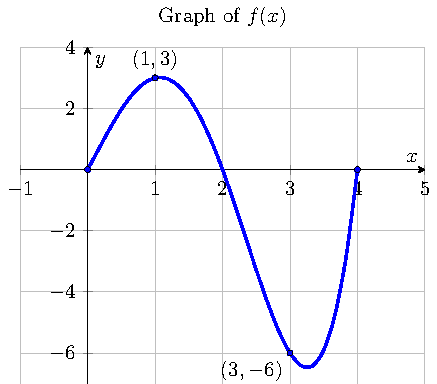
\includegraphics[width=0.9\columnwidth]{figures/0-1-act1.pdf}
\end{center}
\end{minipage}
\begin{minipage}{0.5\columnwidth}
\ba
\item What is the domain of $f(x)$?
\item Approximate the range of $f(x)$.
\item What are  $f(0)$, $f(1)$, $f(3)$, $f(4)$, and $f(5)$?
\ea
\end{minipage}

\end{activity}
\begin{smallhint}
    \ba
        \item The domain is the collection of possible $x$ values.
        \item The range is the collection of possible $y$ values.
        \item Find the $y$ values for each of the given $x$ values.
    \ea
\end{smallhint}
\begin{bighint}
    \ba
        \item The domain should be written as $?? \le x \le ??$.  Look for the smallest
            and largest possible $x$ values.
        \item The range should be written as $?? \le y \le ??$.  Approximate the smallest
            and largest possible $y$ values.
        \item Find the $y$ values for each of the given $x$ values.
    \ea
\end{bighint}
\begin{activitySolution}
   \ba
        \item The domain of $f(x)$ is $0 \le x \le 4$.
        \item The approximate range of $f(x)$ is $-7 \le y \le 3$.  Without the function
            itself we cannot be sure of the actual heights of the function at the maximum
            and the minimum.
        \item $f(0) = 0$, $f(1) = 3$, $f(3) = -6$, $f(4) = 0$, and $f(5)$ does not exist
            since $5$ is not in the domain of $f(x)$.
   \ea
\end{activitySolution}
\aftera


\bex
Find the domain and range of the functions
\[ f(x) = \sin(x), \quad g(x) = \sqrt{x}, \quad \text{and} \quad h(x) =
    \frac{1}{x}. \]
\eex
For $f(x)=\sin(x)$ we recall that the sine function is defined for every possible value of $x$ but
the output is strictly between $y=-1$ and $y=1$.  Therefore, the domain for $f(x) =
\sin(x)$ is $-\infty < x < \infty$ and the range is $-1 \le y \le 1$.  See the left plot
in Figure \ref{f:0.1ex1}.

For $g(x) = \sqrt{x}$ we recall that the square root of a negative number results in an
imaginary number.  In this text we are interested in real-valued output for functions so
we must omit all of the negative numbers from the domain and hence $0 \le x < \infty$.
For the range we recall that the square root of a number will always be a non-negative
number.  As such, the range is $0 \le y < \infty$.  See the middle plot
in Figure \ref{f:0.1ex1}.

For $h(x) = \frac{1}{x}$ we recall that division by zero is mathematically impossible.
That is the only troublesome point in the domain so $-\infty < x < 0$ or $0 < x < \infty$.
A moment's reflection also reveals that it is impossible to get zero out of the function
$h(x)$ but it is possible to get any other number.  Hence $-\infty < y < 0$ or $0 < y <
\infty$. See the right plot in Figure \ref{f:0.1ex1}. 
\afterex

\begin{figure}
    \begin{center}
        \begin{tikzpicture}[scale=0.65]
            \begin{axis}[axis lines=center, title={$f(x) = \sin(x)$}, domain=-6.28:6.28,
                ymin=-1.1, ymax = 1.1, grid]
                \addplot[smooth, very thick, blue] {sin(deg(x))};
            \end{axis}
        \end{tikzpicture}
        \begin{tikzpicture}[scale=0.65]
            \begin{axis}[axis lines=center, title={$g(x) = \sqrt{x}$}, domain=-1:4,
                ymin=-0.5, ymax = 2.5, xmin=-1, grid]
                \addplot[smooth, very thick, red, samples=100] {sqrt(x)};
            \end{axis}
        \end{tikzpicture}
        \begin{tikzpicture}[scale=0.65]
            \begin{axis}[axis lines=center, title={$h(x) = 1/x$},
                ymin=-2, ymax = 2, grid]
                \addplot[smooth, very thick, domain=-3:-0.1, black] {1/x};
                \addplot[smooth, very thick, domain=0.1:3, black] {1/x};
            \end{axis}
        \end{tikzpicture}
    \end{center}
    \caption{Graphs of the function $f(x) = \sin(x)$, $g(x) = \sqrt{x}$, and $h(x) =
    \frac{1}{x}$.}
    \label{f:0.1ex1}
\end{figure}

\subsection*{Slope and Linear Functions}
In Calculus we are often interested in writing the equation for a linear function.  As
such, we should review the features of linear functions.  Every linear function is
characterized by a constant rate of change; the slope.  The slope of a linear function is
a measure of the ``steepness'' of the line.  We use the symbols $\Delta x$,
$\Delta y$ which
mean respectively the ``change in $x$'' and the ``change in $y$''.  
\begin{definition}
    The {\bf slope}, $m$ of a (non-vertical) linear function $f$ which passes through any
    two points $(x_1,y_1)$, $(x_2,y_2)$ can be found using the formula
    \[ m = \frac{\Delta y}{\Delta x} = \frac{y_2 - y_1}{x_2 - x_1} =
    \frac{f(x_2)-f(x_1)}{x_2-x_1} = \frac{\text{Rise}}{\text{Run}} \]
\end{definition}

\begin{minipage}{0.4\columnwidth}
    Recall that
\begin{itemize}
    \item if the line rises from left to right then the slope is positive,
    \item if the line falls from left to right then the slope is negative,
    \item if the line is horizontal then the slope is zero, and
    \item if the line is vertical then the slope is undefined.
\end{itemize}
\end{minipage}
\begin{minipage}{0.5\columnwidth}
    \begin{center}
        \begin{tikzpicture}[scale=0.8]
            \draw[<->, thick] (-4,0) -- (4,0) node[anchor=west]{$x$};
            \draw[<->, thick] (0,-2) -- (0,4) node[anchor=south]{$y$};
            \draw[<->, very thick, blue] (-4,3) -- (4,-1) node[anchor=west]{Negative
            Slope};
            \draw[<->, very thick, color=red, dashed] (-4,-2) -- (4,3)
            node[anchor=west]{Positive Slope};
            \draw[<->, very thick, color=black, dotted] (-4,2) -- (4,2)
            node[anchor=west]{Zero Slope};
        \end{tikzpicture}
    \end{center}
\end{minipage}\bigskip

Depending on the information given there are several convenient forms of the equation of a
line.  Given the definition of the slope
\[ m = \frac{y_2 - y_1}{x_2 - x_1} \]
and letting $(x,y) = (x_2,y_2)$ be any arbitrary point we get the point-slope form of a
linear function.
\begin{definition}
If the linear function $f$ has slope $m$ and passes through the
point $(x_1,y_1)$, then the {\bf point-slope form of the equation of a line} is given by: 
\[ y-y_1=m(x- x_1).  \]
\end{definition}

An alternate form of a linear function which is probably very familiar to most readers is
the slope-intercept form of a line.
\begin{definition}
If the linear function $f$ has slope $m$ and $y$-intercept $b$, then the
{\bf slope-intercept form of the equation of a line} is given by: 
\[ y=mx + b.  \]
\end{definition}
In a calculus class the point-slope form is often the most useful. The
symbols and geometry used in each of the above definitions are shown in Figure
\ref{fig:0.1.linear_fn}.

\begin{figure}[ht!]
    \centering
    \begin{tikzpicture}
        \draw[color=gray!50] (-4,-2) grid (4,4);
        \draw[<->, thick] (-4,0) -- (4,0) node[anchor=west]{$x$};
        \draw[<->, thick] (0,-2) -- (0,4) node[anchor=south]{$y$};
        \draw[<->, very thick, blue] (-4,3) -- (4,-1);
        \draw[color=black, fill=black] (-3.5,2.75) circle(0.075cm) node[anchor=south
        west]{$(x_1,y_1)$};
        \draw[color=black, fill=black] (-1,1.5) circle(0.075cm) node[anchor=south
        west]{$(x_2,y_2)$};
        \draw[color=black, fill=black] (0,1) circle(0.075cm) node[anchor=south
        west]{$(0,b)$};
        \draw[thick, dashed] (-3.5,2.75) -- (-3.5,1.5) -- (-1,1.5);
        \draw (-3.5,2.25) node[anchor=east]{Rise$=\Delta y$};
        \draw (-2,1.5) node[anchor=north]{Run$=\Delta x$};
    \end{tikzpicture}
    \caption{Anatomy of a linear function.}
    \label{fig:0.1.linear_fn}
\end{figure}


\begin{activity}\label{A:0.1.2}
Find an equation of the line with the given information.
\ba
\item The line goes through the points $(-2,5)$ and $(10,-1)$.
\item The slope of the line is $3/5$ and it goes through the point $(2,3)$.
\item The $y$-intercept of the line is $(0,-1)$ and the slope is $-2/3$.
\ea

\end{activity}\aftera


\bex
Write the equation of the line going through the points $(5,7)$ and $(-3,2)$.
\eex
First we calculate the slope 
\[ m = \frac{\Delta y}{\Delta x} = \frac{7 - 2}{5-(-3)} = \frac{5}{8}. \]
Since we have two points and neither is the $y$ intercept of the linear function we choose
to use the point-slope form of the line.  Letting $(x_1,y_1) = (5,7)$ we see that
\[ y - 7 = \frac{5}{8} \left( x-5 \right) \]
is one form of the linear function.  
It is often conventient to solve for $y$ giving us
\[ y = \frac{5}{8} \left( x-5 \right) + 7. \]
Notice that we do not necessarily need to simplify all the way to the slope-intercept form
of the line.  
\afterex

\subsection*{Linear Functions From Data}
A feature of every linear function is that the slope is the same no matter where you are
on the line.  When given a table of data that you suspect might represent a linear
function the slope manifests itself as a constant common difference between successive
$y$-values.  

\bex
Consider the data in the table below.
\begin{center}
    \begin{tabular}[h!]{|c||c|c|c|c|c|}
        \hline
        $x$ & 5 & 6 & 7 & 8 & 9 \\ \hline
        $y$ & 12.2 & 17.5 & 22.8 & 28.1 & 33.4 \\ \hline
    \end{tabular}
\end{center}
Demonstrate that this data is linear and write an equation that fits the data.
\eex
The common differences can be found for each successive $y$-values
\begin{center}
    \begin{tabular}[h!]{|c||c|c|c|c|c|}
        \hline
        $x$ & 5 & 6 & 7 & 8 & 9 \\ \hline
        $y$ & 12.2 & 17.5 & 22.8 & 28.1 & 33.4 \\ \hline
        Common Difference & $\frac{17.5-12.2}{6-5} = 5.3$ & $\frac{22.8-17.5}{7-6} = 5.3$
        & $\frac{28.1-22.8}{8-7} = 5.3$ & $\frac{33.4-28.1}{9-8}=5.3$ & - \\ \hline
    \end{tabular}
\end{center}
The successive differences are clearly the same throughout the data set and the slope for
this data set is $m=5.3$.  Picking any convenient point, say $(5,12.2)$, then allows us to write the
equation of the line as 
\[ y - 12.2 = 5.3(x-5). \]
This could be simplified to point-slope form, but there is typically no need for this
algebraic simplification.
\afterex


\begin{activity}\label{A:0.1.3}
An apartment manager keeps careful record of the rent that he charges as well as the
number of occupied apartments in his complex.  The data that he has is shown in the table
below.  
\begin{center}
    \begin{tabular}{|c||c|c|c|c|c|c|}
        \hline
        Monthly Rent & \$650 & \$700 & \$750 & \$800 & \$850 & \$900 \\
        \hline
        Occupied Apartments & 203 & 196 & 189 & 182 & 175 & 168 \\ \hline
    \end{tabular}
\end{center}

\ba 
\item Just by doing simple arithmetic justify that the function relating the number of occupied
    apartments and the rent is linear.
\item Find the linear function relating the number of occupied apartments to the rent.
\item If the rent were to be increased to \$1000, how many occupied apartments would the
    apartment manager expect to have?
\item At a \$1000 monthly rent what net revenue should the apartment manager expect?
\ea
\end{activity}
\begin{smallhint}
   \ba
        \item Recall what we know about slope on a linear function.
        \item Use the point slope form of the line.  You should have found the slope in
            part (a).
        \item Use your answer to part (b).
        \item How do you get the accumulated payments from all of the tenants?
   \ea
\end{smallhint}
\begin{bighint}
   \ba
        \item Check that the slope is constant.
        \item Use the first two points in the point slope form of the line.
        \item Once you have the linear function from part (b), substitute \$1000 in for
            the rent.
        \item We are looking for the rent accumulated by all of the tenants.
   \ea
\end{bighint}
\begin{activitySolution}
   \ba
        \item The slope is 
            \[ m = \frac{196-203}{700-650} = -\frac{7}{50} \]
            and this slope is consistent no matter which pairs of points we choose.
        \item Let $A$ be the number of occupied apartments and let $R$ be the rent.  The
            linear function relating the number of occupied apartments and the rent is
            \[ A - 203 = -\frac{7}{50} \left( R - 650 \right). \]
            Solving for $A$ we get
            \[ A(R) = -\frac{7}{50} \left( R - 650 \right) + 203. \]
            This is a perfectly acceptable algebraic form for the answer, but if you
            insist on simplifying then
            \[ A(R) = -\frac{7}{50} R + 294. \]
        \item $A(1000) = -\frac{7}{50} \left( 1000 - 650 \right) + 203 = 252$ units
            occupied.
        \item The net revenue is the product of the monthly rent and the number of units
            occupied at that rent.  In this case the revenue is $\$1000 \cdot 252 =
            \$252,000$.
   \ea
\end{activitySolution}
\aftera



\bex
The Old Farmer's Almanac tells us that you can tell the temperature by counting the chirps
of a cricket.  It is a linear function $T=f(C)$ given by $T$ (in degrees Fahrenheit)=\# of
chirps in 15 seconds $+40$.  We can approximate this with the formula 
\[ T =  \frac{C}{4} + 40 \]
where $C$ is the number of chirps/minute and $T$ is in $^\circ F$.
\ba
    \item If the chirp rate is 120 chirps/minute, what is the temperature?
    \item Suppose that crickets will not chirp if the temperature is below $56^\circ F$.
        We can also suppose that crickets will not chirp above $136^\circ F$ since that is
        the highest temperature ever recorded at a weather station.  With these
        parameters, what is the domain of this function?
\ea
\eex
\ba
    \item If $C = 120$ chirps/minute, substitute this into the function $T(C)$ to obtain
        \[ T(120) = \frac{120}{4} + 40 = 30 + 40 = 70^\circ F. \]
    \item To find the domain we need to find the appropriate values of $C$ for the $T(C)$
        function.  Solve $56=C/4+40$ and get $C = 64$.  Solve $136=C/4+40$ and get $C =
        384$.  So the domain of $T(C)$ is $64 \le \text{chirps/minute} \le 384$ or, in
        interval notation, $[64, 136]$. 

\ea
\afterex


\subsection*{Families of Linear Functions}
We noted above that a linear function has the form  $y=f(x)=mx+b$, where $m$ is the slope of
the line, and $b$ is the $y$-intercept.  Since $m$ and $b$ can take on various values, taken
together, they represent a family of functions.  For example, we could fix $b = 2$, and then
draw the graphs of $f(x)=mx+2$ for various values of $m$; for example, $m = -1, -2, 2, 1$.
Doing so would give the functions in the family $f(x)=mx+2$ shown in the left image of Figure
\ref{fig:0.1.fam1}.

Similarly, we could set $m$ to be $2$ and let $b$ take on the values $b=-1, 1, 4, -6$ and
we would get
some examples from the family of functions for $y=f(x)=2x+b$ shown in the right image of Figure
\ref{fig:0.1.fam1}.


From the right image in Figure \ref{fig:0.1.fam1} it should be clear to the reader that
parallel lines have the same slope.  What can you say about the slopes of perpendicular
lines?  Here is the result that we state without proof.
\begin{theorem}\label{thm:test}
If line $\ell_1$ has slope $m_1$ and line $\ell_2$ has slope $m_2$, then 
    \begin{itemize}
        \item lines $\ell_1$ and $\ell_2$ are parallel if the slopes are the same: $m_1 = m_2$,
            and
        \item lines $\ell_1$ and $\ell_2$ are perpendicular if the slopes are opposite
            reciprocals: $m_2 = -\frac{1}{m_1}$.
    \end{itemize}
\end{theorem}

\def\scl{0.8}
\begin{figure}[ht]
    \centering
    \begin{tikzpicture}[scale=\scl]
        \begin{axis}[axis lines=center, xmin=-5, xmax=5, ymin=-10, ymax=10,
            legend style={ at={(axis cs:4.03,5)}, anchor=west }]
            \addplot[smooth, very thick, color=blue] {-1*x+2};
            \addlegendentry{$y=-x+2$};
            \addplot[smooth, very thick, color=red, dashed] {-2*x+2};
            \addlegendentry{$y=-2x+2$};
            \addplot[smooth, very thick, color=cyan, dotted] {1*x+2};
            \addlegendentry{$y=x+2$};
            \addplot[smooth, very thick, color=black] {2*x+2};
            \addlegendentry{$y=2x+2$};
        \end{axis}
    \end{tikzpicture}
    \begin{tikzpicture}[scale=\scl]
        \begin{axis}[axis lines=center, xmin=-5, xmax=5, ymin=-10, ymax=10,
            legend style={ at={(axis cs:4.03,5)}, anchor=west }]
            \addplot[smooth, very thick, color=blue] {2*x-1};
            \addlegendentry{$y=2x-1$};
            \addplot[smooth, very thick, color=red, dashed] {2*x+1};
            \addlegendentry{$y=2x+1$};
            \addplot[smooth, very thick, color=cyan, dotted] {2*x+4};
            \addlegendentry{$y=2x+4$};
            \addplot[smooth, very thick, color=black] {2*x-6};
            \addlegendentry{$y=2x-6$};
        \end{axis}
    \end{tikzpicture}
    \caption{Several members of the family of linear functions $f(x) = mx+2$ (left) and
    the family $f(x) = 2x+b$ (right).}
    \label{fig:0.1.fam1}
\end{figure}

\begin{activity}\label{A:0.1.4}
Write the equation of the line with the given information.
\ba
\item Write the equation of a line parallel to the line $y=\frac{1}{2}x+3$ passing through
    the point $(3,4)$.
\item Write the equation of a line perpendicular to the line $y=\frac{1}{2}x + 3$ passing
    through the point $(3,4)$.
\item Write the equation of a line with $y$-intercept $(0,-3)$ that is perpendicular to
    the line $y=-3x-1$.
\ea
\end{activity}\aftera



% \subsection*{Equations, Functions, and Expressions}
% To conclude this first section we define three commonly misused mathematical terms.
% \begin{definition}
%     A {\bf mathematical expression} is a combination of numbers, variables, and operations
%     (addition, subtraction, multiplication, roots, etc).  Several examples are:
%     \begin{itemize}
%         \item $2x+3$
%         \item $\sqrt{a^2 + b^2}$
%         \item $\pi r^2$
%     \end{itemize}
% \end{definition}
% 
% \begin{definition}
%     An {\bf equation} is a mathematical statement containing an equal sign where the left
%     and right-hand sides of the equal sign are expressions in the same variable.  Examples
%     are:
%     \begin{itemize}
%         \item $3=5x-2$
%         \item $x^2-2x+5=9$
%         \item $\sqrt{3x-2} = 19$
%     \end{itemize}
% \end{definition}
% 
% \begin{definition}
%     A {\bf function} (as defined before) is a rule that associates a value $x$ in the
%     domain to a value $y$ in the range.  Examples include:
%     \begin{itemize}
%         \item $y=x^2+3$
%         \item $f(x) = 3x-4$
%         \item $f(y) = \sqrt{3y-2}$
%     \end{itemize}
% \end{definition}
% 
% It is easy for students to confuse the meanings of these three definitions, so here are
% some helpful tips:
% \begin{itemize}
%     \item If there is no equal sign then it is an expression.
%     \item It makes sense to substitute a value into an expression, but saying that you're
%         going to ``solve'' an expression is meaningless.
%     \item If it is an equation then it is meaningful to ``solve'' the equation.  It is NOT
%         meaningful to say that you are going to ``solve'' a function or expression.
%     \item A function defines a rule that associates two variables.
%     \item A function has an associated graph whereas expressions and equations do not.
% \end{itemize}
% 
% \begin{activity}\label{A:0.1.5}
    Classify each of the following as an expression, equation, or a function.  For each
    function, classify it as either linear or non-linear.  Finally, for each linear
    function find the slope and $y$-intercept.
    \ba
    \item $y=6y-3$
    \item $y=6x-3$
    \item $6x-3$
    \item $-4y+2x+8=0$
    \item $12x=6y+4$
    \item $12x=6y^2+4$
    \item $\sqrt{x+2}$
    \item $y=\sqrt{x+2}$
    \item $x=\sqrt{x+2}$
    \item $x^2+2x-3$
    \item $x+2x-3=9$
    \ea

\end{activity}\aftera

% 
% % more activites

\begin{summary}
\item A function assigns one $y$ value to each $x$ value.
\item The slope of a linear function can be written as 
    \[ m = \frac{\text{Rise}}{\text{Run}} = \frac{y_2 - y_1}{x_2 - x_2} \]
\item A linear function can be written in the forms
    \[ y = mx + b \quad \text{or} \quad y-y_1 = m(x-x_1) \]
\item When examining linear data, the differences between successive $y$-values reveals
    the slope.
\end{summary}

\nin \hrulefill

% exercises go here
\begin{exercises} 

\item (modified from NCTM Illuminations) The table below displays data that relate the number of oil changes per year and the
    cost of engine repairs.  To predict the cost of repairs from the number of oil
    changes, use the number of oil changes as the $x$ variable and the engine repair cost
    as the $y$ variable.  
    \begin{center}
        \begin{tabular}[h!]{|c|c|}
            \hline
            Oil Changes Per Year & Cost of Repairs (\$) \\ \hline \hline
            3 & 300 \\ 
            5 & 300 \\ 
            2 & 500 \\
            3 & 400 \\ 
            1 & 700 \\
            4 & 400 \\
            6 & 100 \\
            4 & 250 \\ 
            3 & 450 \\
            2 & 650 \\
            0 & 600 \\ 
            10 & 0 \\
            7 & 150 \\ \hline
        \end{tabular}
    \end{center}

    \ba
    \item Using graph paper make a plot of the data on appropriate axes.
    \item Do the data appear linear?  Why or why not?
    \item Pick two representative points from the data and use them to write the
        equation of a line that {\it fits} the data.  Plot your line on top of your data
        and discuss how well your line fits the
        data.   (This may take a few attempts.)
    \item Despite how well your data fit a linear model, it is not entirely sensible to
        use a linear model for this data.  Why?
    \ea
    
\begin{exerciseSolution}
\end{exerciseSolution}


\item The population of a city, $P$, in millions, is a function of $t$, the number of
    years since 1960, so $P = f(t)$.  Which of the following statements explains the
    meaning of $f(38) = 8$ in terms of the population of this city?
    \ba
        \item The population of this city in the year 38 is 8 million people.
        \item The population of this city in the year 8 is 38 million people.
        \item The population of this city in the year 1968 is 38 million people.
        \item The population of this city in the year 1998 is 8 million people.
    \ea
\begin{exerciseSolution}
    The independent variable is the number of years after 1960 so the ``38'' represents
    the year 1998.  Hence, the phrase ``The population of this city in the year 1998 is 8
    million people'' is the correct phrase.
\end{exerciseSolution}

\item Determine the slope and $y$-intercept of the line whose equation is $-4y + 6x + 8 =
    0$.

\begin{exerciseSolution}
    Solving for $y$ we see that 
    \[ 4y = 6x + 8 \quad \implies \quad y = \frac{6}{4} x + 2. \]
    Therefore the slope is $m=\frac{6}{4} = \frac{3}{2}$ and the $y$-intercept is $2$.
\end{exerciseSolution}

\item The value of a car in 1990 is \$13,100 and the value is expected to go down by \$80
    per year for the next 7 years.  Write a linear function for the value, $V$, of the
    1990 car as a function of the number of years from 1990, $x$.  

\begin{exerciseSolution}
    \[ V(x) = -80x + 13100 \] 
\end{exerciseSolution}
\end{exercises}
\afterexercises







\clearpage


\section{Exponential Functions} \label{S:0.2.Exponentials}


\vspace*{-14 pt}
\framebox{\hspace*{3 pt}
\parbox{6.25 in}{\begin{goals}
\item How can exponential functions be used to model growth and decay of populations,
    investments, radioactive isotopes, and many other physical phenomena?
\item How can we build exponential functions from data?
\end{goals}} \hspace*{3 pt}}


% \begin{web}
% \item
%     \href{https://www.khanacademy.org/math/algebra2/exponential_and_logarithmic_func/exp_growth_decay/v/exponential-growth-functions}{Khan
%     Playlist: Exponential growth and decay}
% \item
%     \href{https://www.khanacademy.org/math/algebra2/exponential_and_logarithmic_func/exponential-modeling}{Khan
%     Playlist: Modeling with exponential functions}
% \item
%     \href{https://www.khanacademy.org/math/algebra2/exponential_and_logarithmic_func/continuous_compounding}{Khan
%     Playlist: Continuous compounding interest}
% \end{web}

\nin \hrulefill


\subsection*{Introduction}
The exponential function is a powerful tool in the mathematician's arsenal for modeling
growth and decay phenomena.  The common applications of the exponential funciton range
from population modeling, to tracking drug levels in the blood stream, to using carbon
dating to estimate the age of an artifact.  The common mathematical fact about all of
these situations is that the growth (or decay) rate is a constant multiple.  For example,
if we are measuring exponential population growth then the ratio of two successive
populations must be constant.  Linear functions have a similar behavior, except that in
linear functions the difference (not the ratio) between two successive values is constant
(the slope).  


\begin{pa} \label{PA:0.2}
Suppose that the populations of two towns are both growing over time.  The town of
Exponentia is growing at a rate of 2\% per year, and the town of Lineola is growing at a
rate of 100 people per year.  In 2014, both of the towns have 2,000 people.
\ba
    \item Complete the table for the population of each of these towns over the next
        several years.
        \begin{center}
            \begin{tabular}[h!]{|c|c|c|c|c|c|c|c|c|c|c|c|}
                \hline
                & 2014 & 2015 & 2016 & 2017 & 2018 & 2019 & 2020 & 2021 & 2022 \\ \hline
                Exponentia & 2000 & & & & & & & & \\ \hline
                Lineola &  2000 & & & & & & & & \\ \hline
            \end{tabular}
        \end{center}
    \item Write a linear function for the population of Lineola. Interpret the slope in
        the context of this problem.
    \item The ratio of successive populations for Exponentia should be equal.  For
        example, dividing the population in 2015 by that of 2014 should give the same
        ratio as when the population from 2016 is divided by the population of 2015.  Find
        this ratio.  How is this ratio related to the 2\% growth rate?
    \item Based on your data from part (a) and your ratio in part (c), write a function
        for the population of Exponentia.
    \item When will the population of Exponentia exceed that of Lineola?
\ea
\end{pa} \afterpa


\subsection*{Exponential Functions}
Consider the example where the population of a bacteria colony is doubling every week.  If
in the first week there are 100 bacteria, then there are 200 bacteria by the end of the
second week, 400 by the end of the third and so on.  In Table \ref{tab:0.2.bacteria} and
Equation \eqref{eqn:0.2.bacteria} we can see a simple way to model this type of growth. 
\begin{table}[h!]
    \centering
    \begin{tabular}{|c|c|}
        \hline
        Week & Bacteria \\ \hline
        0 &  $100$ \\
        1 &  $100 \cdot 2=200$ \\
        2 &  $200 \cdot 2 = 100 \cdot 2^2=400$ \\
        3 &  $400 \cdot 2 = 100 \cdot 2^3=800$ \\
        \vdots & \vdots \\ \hline
    \end{tabular}
    \caption{Bacteria population doubling}
    \label{tab:0.2.bacteria}
\end{table}
\begin{flalign}
    P(t) = 100 \cdot 2^t \quad \text{($t=$ number of weeks)}
    \label{eqn:0.2.bacteria}
\end{flalign}

The time, $t$ in equation \eqref{eqn:0.2.bacteria} is measured in weeks.  It is easy to see that
the ratio of the populations for each successive week is constant at $P(t+1)/P(t) = 2$.
This is indicative of exponential growth.  Of course, this population growth could have
been modeled using time measured in days instead.  The population still doubles every week
so for this new model the value at $t=7$ should be double the value at $t=0$.  Equation
\eqref{eqn:0.2.bacteria_days} shows this new model with only a slight modification
adjusting for the new time measurement.
\begin{flalign}
    P(t) = 100 \cdot 2^{t/7} \quad \text{($t=$ number of days)} 
    \label{eqn:0.2.bacteria_days}
\end{flalign}

This type of modeling and thought process can be used to describe most exponential growth
and decay situations.  One
general formula for an exponential function is 
\begin{flalign}
    f(x) = A \cdot r^{kx}.
    \label{eqn:0.2.exponential}
\end{flalign}
where $A$ is some given initial value, $r$ is the common ratio, and $k$ is a constant
given by the frequency in which the common ratio is applied.  In the previous population
doubling example, $A=100$, $r=2$, and $k=1/7$.

% \begin{callout}
    A few simple guidelines should make it clear when an exponential function is modeling
growth or decay.  
\begin{itemize}
    \item If $r > 1$ then the function exhibits exponential growth.
    \item If $0 < r < 1$ then the function exhibits exponential decay.
    \item If a population is growing by $p\%$ per unit time, then $r = 1+p/100$.
    \item If a population is decreasing by $p\%$ per unit time, then $r = 1-p/100$.
\end{itemize}
% \end{callout}

\begin{activity}\label{A:0.2.1}
    Consider the exponential functions plotted in Figure \ref{F:0.2.Act1}
    \ba
        \item Which of the functions have common ratio $r > 1$?
        \item Which of the functions have common ratio $0<r< 1$?
        \item Rank each of the functions in order from largest to smallest $r$ value.
    \ea
    \begin{figure}[h!]
        \begin{center}
            \begin{tikzpicture}
                \begin{axis}[axis lines=center, xlabel={$x$}, ylabel={$y$}, xmin=-3, xmax=3,
                    ymin=-1, ymax=5, domain=-3:3,legend pos=outer north east]
                    \addplot[smooth, blue, very thick] {2^x};
                    \addlegendentry{$f(x)$};
                    \addplot[smooth, red, very thick, dashed] {3^x};
                    \addlegendentry{$g(x)$};
                    \addplot[smooth, green!50!black, very thick, dotted] {1.5^x};
                    \addlegendentry{$h(x)$};
                    \addplot[smooth, black, very thick, dashdotted] {(0.5)^x};
                    \addlegendentry{$k(x)$};
                    \addplot[smooth, cyan, very thick, densely dotted] {(0.9)^x};
                    \addlegendentry{$m(x)$};
                \end{axis}
            \end{tikzpicture}
        \end{center}
        \caption{Exponential growth and decay functions} \label{F:0.2.Act1}
    \end{figure}
\end{activity}\aftera



\bex
One application to exponential decay is to calculate the intensity of radiation from
radioactive isotopes.  Most isotopes emit particles and decay into stable forms.  We
measure the rate of decay from the particles by the isotope's half-life, which is
how long it takes half of the isotope to decay.  The half-life for Sodium-25 ($Na^{25}$)
is almost exactly one minute.  Write a function that models that amount of $Na^{25}$ over
time if you start with exactly 36 grams.    
\eex
If you begin with 36 grams of $Na^{25}$ then the number of
grams remaining after $t$ minutes, $S(t)$, can be represented by the function
\[ S(t) = 36 \left( \frac{1}{2} \right)^{t}, \]
where $t$ is measured in minutes. Figure \ref{F:0.2.Ex1} shows this exponential decay
function with an initial value of 36 and a value of 18 after 1 day.
\begin{figure}[ht!]
    \begin{center}
%         \begin{tikzpicture}
%             \begin{axis}[axis lines=center, xlabel={$t$ (minutes)}, ylabel={$S(t)$
%                 (grams)}, xmin=0, xmax=5,ymin=0, ymax=40, domain=0:5]
%                 \addplot[blue, very thick, smooth] {36*(0.5)^x};
%                 \addplot[mark=*,red,very thick] coordinates{(1,18)};
%                 \addplot[mark=*,blue,very thick] coordinates{(0,36)};
%                 \draw (axis cs:1,18) node[anchor=west]{$(1,18)$};
%             \end{axis}
%         \end{tikzpicture}
        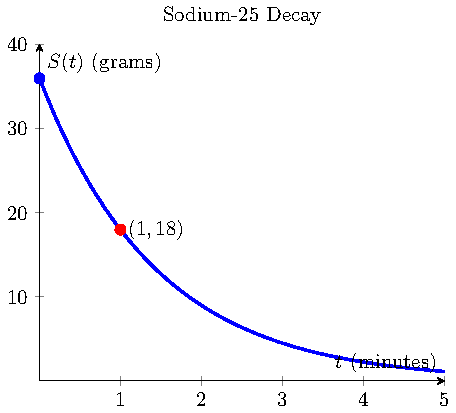
\includegraphics[width=0.5\columnwidth]{figures/0-2-fig2.pdf}
    \end{center}
    \caption{The grams of Sodium-25 remaining as a function of time. The blue point
    represents the initial value $(0,36)$ and the red point represents the value after 1
minute $(1,18)$.}
    \label{F:0.2.Ex1}
\end{figure}
\afterex

% \bigskip
\begin{activity}\label{A:0.2.2}
    A sample of $Ni^{56}$ has a half-life of 6.4 days.  Assume that there are 30 grams
    present initially.
    \ba
        \item Write a function describing the number of grams of $Ni^{56}$ present as a
            function of time.  Check your function based on the fact that in 6.4 days
            there should be 50\% remaining.
        \item What percent of the substance is present after 1 day?
        \item What percent of the substance is present after 10 days?
    \ea
\end{activity}
\begin{smallhint}
   \ba
        \item The growth rate should be $1/2$.
        \item Figure out how much is there after 1 day and divide by the original amount.
        \item Figure out how much is there after 10 days and divide by the original amount.
   \ea
\end{smallhint}
\begin{bighint}
   \ba
        \item When you substitute $6.4$ for the time you should have decayed by exactly
            half.
        \item Figure out how much is there after 1 day and divide by the original amount.
        \item Figure out how much is there after 10 days and divide by the original amount.
   \ea
\end{bighint}
\begin{activitySolution}
   \ba
        \item $A(t) = 30 \left( \frac{1}{2}  \right)^{t/6.4}$
        \item $A(1) =  30 \left( \frac{1}{2}  \right)^{1/6.4} \approx 26.9206$ so the
            percent that remains is just shy of 90\%.
        \item $A(10) =  30 \left( \frac{1}{2}  \right)^{10/6.4} \approx 10.1569$ so the
            percent that remains is about 33.9\%.
   \ea
\end{activitySolution}

\aftera


% \bigskip
\begin{activity}\label{A:0.2.3}\cite[p.9]{nonlinear}
    Uncontrolled geometric growth of the bacterium {\it Escherichia coli (E. Coli)} is the
    theme of the following quote taken from the best-selling author Michael Crichton's
    science fiction thriller, {\it The Andromeda Strain:}
    \begin{quote}
        ``The mathematics of uncontrolled growth are frightening.  A single cell of the
        bacterium E. coli would, under ideal circumstances, divide every twenty minutes.
        That is not particularly disturbing until you think about it, but the fact is that
        that bacteria multiply geometrically: one becomes two, two become four, four
        become eight, and so on.  In this way it can be shown that in a single day, one
        cell of E. coli could produce a super-colony equal in size and weight to the
        entire planet Earth.''
    \end{quote}
    \ba
        \item Write an equation for the number of E. coli cells present if a single cell
            of E. coli divides every 20 minutes. 
        \item How many E. coli would there be at the end of 24 hours?
        \item The mass of an E. coli bacterium is $1.7 \times 10^{-12}$ grams, while the
            mass of the Earth is $6.0 \times 10^{27}$ grams.  Is Michael Crichton's claim
            accurate?  Approximate the number of hours we should have allowed for this
            statement to be correct?
    \ea
\end{activity}\aftera


\subsection*{Investments}
Interest bearing bank accounts and investments follow exponential growth and decay models.
In the case of a savings account the interest is typically compounded several times per
year.  This means that the investor is getting interest on their interest every time the
bank computes the interest.    

% \begin{callout}
    If the money is gaining $p\%$ interest compounded $n$ times per year then the common ratio
for the exponential function is $1 + p/n$.  The exponent needs to reflect the fact that
the interest occurs at monthly intervals.  This means that the exponential function is
\begin{flalign}
    A(t) = A_0 \left( 1+\frac{p}{n} \right)^{nt} \quad \text{($t=$ number of years)}.
    \label{eqn:0.2.compound_interest}
\end{flalign}
In Equation \eqref{eqn:0.2.compound_interest}, $A_0$ is the initial investment, $A(t)$ is
the value of the investment over time, $p$ is the interest rate, and $n$ is the number of
times the interest is compounded per year.
% \end{callout}

\bex\label{0.2.Ex2}
If \$100 are invested into a bank account earning 2\% interest compounded 12 times per
year, how much does the investor have at the end of 1 year? 5 years? at retirement age?
How does this change is we compound quarterly or daily instead of monthly?
\eex
In the present situation the function modeling the value of the investment is
\[ A(t) = 100 \left( 1 + \frac{0.02}{12} \right)^{12t}. \]
Table \ref{tab:0.2.ex2} shows the value of the investment over the first 5 years.  It is
clear that this is very slow growth, but it is exponential none the less.  The common
ratio in this case is $r = (1+0.02/12) \approx 1.0017$, and this means that you are really
gaining 0.17\% interest per month.
\begin{table}[ht!]
    \centering
    \begin{tabular}{|c|c|c|c|c|c|c|}
        \hline
        Year & 0 & 1 & 2 & 3 & 4 & 5 \\ \hline
        Value & \$100 & \$102.02 & \$104.08 & \$106.18 & \$ 108.32 & \$ 110.51 \\ \hline
    \end{tabular}
    \caption{Value of \$100 investment for the first 5 years}
    \label{tab:0.2.ex2}
\end{table}

Assume that our investor was an 18 year old and extrapolate this to retirement age,
let's say 65 years old.  That is 47 years worth of interest, and the initial \$100
investment becomes 
\[ A(47) = 100 \left( 1 + \frac{0.02}{12} \right)^{12\cdot 47} \approx \$256. \]

If the number of times the bank compounds the interest changes the function will still
have essentially the same form: $A(t) = 100 (1+\frac{0.02}{n})^{nt}$. In Table
\ref{tab:0.2.ex2_n} the same investment is considered for several values of $n$.  While
more compoundings per year generally gives a higher rate of return on the investment, the
impact is small for larger values of $n$.  
\begin{table}[ht!]
    \centering
    \begin{tabular}{|c|c|c|c|c|c|c|c|c|}
        \hline
        Year & 0 & 1 & 2 & 3 & 4 & 5 & $\cdots$ & 47 \\ \hline
        Value ($n=1$) & \$100 & \$102.00 & \$104.04 & \$106.12 & \$ 108.24 & \$ 110.41 &
        $\cdots$ & \$253.63  \\ \hline
        Value ($n=4$) & \$100 & \$102.02 & \$104.07 & \$106.17 & \$ 108.31 & \$ 110.49 &
        $\cdots$ & \$255.40 \\ \hline
        Value ($n=12$) & \$100 & \$102.02 & \$104.08 & \$106.18 & \$ 108.32 & \$ 110.51 &
        $\cdots$ & \$255.80 \\ \hline
        Value ($n=365$) & \$100 & \$102.02 & \$104.08 & \$106.18 & \$ 108.33 & \$ 110.52 &
        $\cdots$ & \$255.99 \\ \hline
    \end{tabular}
    \caption{Value of \$100 investment for various values of $n$.}
    \label{tab:0.2.ex2_n}
\end{table}
\afterex

\subsection*{Exponential Functions with Base $e$}
Exponential functions are commonly written with a base of $e \approx 2.718281828459045\dots$.
This may seem like an arbitrary and bizarre choice at first glance, but we will see that this famous
number (called Euler's Number \footnote{Euler's number is named after the famous $17^{th}$
century mathematician Leonhard Euler. Euler was the first mathematician to introduce the
notion of a function, and he is responsible for a large amount of the development of
Calculus.}) plays a central role in Calculus.  

Euler's number can be derived from Equation \eqref{eqn:0.2.compound_interest} if we assume
that a fictitious bank gives $100\%$ interest compounded infinitely many times per year on
a one dollar investment.  Mathematically this is written as
\begin{flalign}
    e = 1 \cdot \left( 1 + \frac{1}{n} \right)^n \text{ as } n \to \infty.
    \label{eqn:0.2.euler}
\end{flalign}
\begin{table}[h!]
    \centering
    \begin{tabular}{|c|c|c|c|c|c|c|c|}
        \hline
        $n$ & $1$ & $10$ & $100$ & $1000$ & $\cdots$ & $10^{10}$& $\cdots$  \\ \hline
        $(1+\frac{1}{n})^n$ & $2$ & $2.5935$ & $2.7048$ & $2.7169$ & $\cdots$ & $2.71828$& $\cdots$  \\
        \hline
    \end{tabular}
    \caption{Approximations of Euler's number, $e$, using equation \eqref{eqn:0.2.euler} with various values of $n$}
    \label{tab:0.2.euler}
\end{table}

Any exponential function can be rewritten in terms of Euler's number in the form
\begin{flalign}
    f(x) = A e^{kx}.
    \label{eqn:0.2.exponential_e}
\end{flalign}
% \begin{callout}
In Equation \eqref{eqn:0.2.exponential_e}, $k$ is called the continuous
rate\index{continuous rate}.  
\begin{itemize}
    \item If $k>0$ then $f(x) = Ae^{kx}$ models exponential growth.
    \item If $k<0$ then $f(x) = Ae^{kx}$ models exponential decay.
\end{itemize}
% \end{callout}

\bex
A population of a city is 5000 people and is doubling in size every 5 years.  Use
equations \eqref{eqn:0.2.exponential} and \eqref{eqn:0.2.exponential_e} to write two
different functions modeling this population; one with base 2 and one with base $e$.
\eex
If the population is doubling every 5 years we can use equation
\eqref{eqn:0.2.exponential} to write
\[ P(t) = 5000 \cdot 2^{t/5}. \]
In order to use equation \eqref{eqn:0.2.exponential_e} we need to find the value of
``$k$''.  This is done by using the fact that at year 5 the population will be 10000 and
solving the equation
\[ 10000 = 5000 \cdot e^{5k}. \]
Rearranging we see that $e^{5k} = 2$.  In order to solve this algebraic equation we need
to use logarithms.  These important functions will be discussed in more detail in the
logarithms section %\ref{S:0.4.Logarithms}.  
In this case we see that $k = \ln(2) / 5 \approx 0.139.$
Therefore,
\[ P(t) = 5000 \cdot e^{0.139 t}. \]
Since these two equations model the same population they must be identical.  Indeed,
\[ 5000 \cdot 2^{t/5} = 5000 \cdot \left( 2^{1/5} \right)^t \approx 5000 \cdot (1.149)^t,
\]
and
\[ 5000 \cdot e^{kt} = 5000 \cdot \left( e^k \right)^t \approx 5000 \cdot (1.149)^t. \]
\afterex

% \begin{activity}\label{A:0.2.3}
The quantity, $Q$, of a drug in a patient's body at time $t$ is represented for positive
constants $S$ and $k$ by the function $Q(t) = S(1-e^{-kt})$. 
\ba
\item For $t \ge 0$ describe how $Q(t)$ changes with time.
\item Assuming that $S = 5$, use a graphing utility to make a sketch of $Q(t)$ with
    various values of $k$.  Use the left-hand side of Figure \ref{F:0.2.Act3} to organize
    your plots.  Interpret the value of $k$ in the context of this problem.
\item Now assume that $k=0.5$ and use a graphing utility to make a sketch of $Q(t)$ with
    various values of $S$.  Use the right-hand side of Figure \ref{F:0.2.Act3} to organize
    your plots.  Interpret the value of $S$ in the context of this problem.
\ea
\begin{figure}[h!]
    \begin{center}
        \begin{tikzpicture}
            \begin{axis}[axis lines=center,xlabel={$t$}, ylabel={$Q$}, xmin=0, ymin=0, xmax=6,
                ymax=10, grid, title={$Q(t)$ with $S=5$}]
                \addplot[smooth] {0*x};
            \end{axis}
        \end{tikzpicture}
        \begin{tikzpicture}
            \begin{axis}[axis lines=center,xlabel={$t$}, ylabel={$Q$}, xmin=0, ymin=0, xmax=6,
                ymax=10, grid, title={$Q(t)$ with $k=0.5$}]
                \addplot[smooth] {0*x};
            \end{axis}
        \end{tikzpicture}
    \end{center}
    \caption{Plot for Activity \ref{A:0.2.3}}
    \label{F:0.2.Act3}
\end{figure}
\end{activity}\aftera


% more activites

\begin{summary}
\item An exponential function can be written in the form $f(x) = A r^{kx}$ or $g(x) = A
    e^{kx}$.  
    \begin{itemize}
        \item In $f(x)$, if $k>0$ and $r>1$ then $f(x)$ models exponential growth.
        \item In $f(x)$, if $k>0$ and $0<r<1$ then $f(x)$ models exponential decay.
        \item In $g(x)$, if $k>0$ then $g(x)$ models exponential growth.
        \item In $g(x)$, if $k<0$ then $g(x)$ models exponential decay.
    \end{itemize}
\item Exponential functions have a constant common ratio for successive time values.
\end{summary}

\nin \hrulefill

% exercises go here
\begin{exercises} 

\item Suppose that $h(t) = A \cdot r^t$.  If $h(3)=4$ and $h(5)=40$,
    \ba
        \item find $r$.
        \item find $A$.
        \item Does this function model exponential growth or decay? How can you tell?
    \ea
\begin{exerciseSolution}
\end{exerciseSolution}


\item The half-life of $Br^{77}$ is 57 hours.
    \ba
        \item If the initial amount is $150$ grams, find the amount remaining after 171
            hours.
        \item Write an equation to predict the amount remaining after $t$ hours.
        \item Estimate within one hour how long it will take the amount to decrease to 10
            grams.
    \ea
\begin{exerciseSolution}
\end{exerciseSolution}


\item Consider the data in Table \ref{tab:0.2.exercise3}
    \ba
        \item Which (if any) of the functions could be linear? Explain how you know that
            these functions are linear, and find formulas for these functions.
        \item Which (if any) of the functions could be exponential? Explain how you know
            that these functions are linear, and find formulas for these functions.
    \ea
    \begin{table}[h!]
        \centering
        \begin{tabular}{|c|c|c|c|}
            \hline
            $x$ & $f(x)$ & $g(x)$ & $h(x)$ \\ \hline
           $-2$&$12$&$16$&$37$\\
           $-1$&$17$&$24$&$34$\\
           $0 $&$20$&$36$&$31$\\
           $1 $&$21$&$54$&$28$\\
           $2 $&$18$&$81$&$25$\\ \hline
        \end{tabular}
        \caption{Data tables for $f(x)$, $g(x)$, and $h(x)$}
        \label{tab:0.2.exercise3}
    \end{table}
\begin{exerciseSolution}
\end{exerciseSolution}

\end{exercises}
\afterexercises




\clearpage

\section{Transformations of Functions} \label{S:0.3.Transformations}


\vspace*{-14 pt}
\framebox{\hspace*{3 pt}
\parbox{6.25 in}{\begin{goals}
\item How can new functions be generated by shifts, stretches, and transformations of
    well-known functions?
\item How can we mathematically describe symmetric functions?
\item How can we build inverse functions, and when do those functions exist?
\end{goals}} \hspace*{3 pt}}


% \begin{web}
% \item
%     \href{https://www.khanacademy.org/math/algebra2/functions_and_graphs/shifting-reflecting-functions/v/shifting-and-reflecting-functions}{Khan
%     Playlist: Shifting and reflecting functions}
% \item
%     \href{https://www.khanacademy.org/math/algebra2/functions_and_graphs/analyzing_functions}{Khan
%     Playlist: Analyzing functions}
% \item
%     \href{http://www.geogebratube.org/student/m93018}{Geogebra Applet for function
%     transformations}
% \end{web}

\nin \hrulefill


\subsection*{Introduction}
There are infinitely many functions that can be generated using the basic mathematical
operations (addition, subtraction, multiplication, division, and exponentiation) along
with {\it simple} functions such as roots, exponentials, and trigonometric functions.  In
fact, we can build entire families of functions based only on these simple building
blocks.

\begin{pa} \label{PA:0.3}
The goal of this activity is to explore and experiment with the function
\[ F(x) = Af(B(x-C))+D. \]
The values of $A$, $B$, $C$, and $D$ are constants and the function $f(x)$ will be
henceforth called the {\it parent function}.  To facilitate this exploration, use the
applet located at \\
\href{http://www.geogebratube.org/student/m93018}{http://www.geogebratube.org/student/m93018}.
\ba
    \item Let's start with a simple function.  Let the parent function be $f(x) = x^2$.
        \bei
            \item Fix $B=1$, $C=0$, and $D=0$.  Write a sentence or two describing the
                action of $A$ on the function $F(x)$.
            \item Fix $A=1$, $B=1$, and $D=0$.  Write a sentence of two describing the
                action of $C$ on the function $F(x)$.
            \item Fix $A=1$, $B=1$, and $C=0$.  Write a sentence of two describing the
                action of $D$ on the function $F(x)$.
            \item Fix $A=1$, $C=0$, and $D=0$.  Write a sentence of two describing the
                action of $B$ on the function $F(x)$.
        \eei
    \item Test your conjectures with the functions $f(x) = |x|$ (typed \texttt{abs(x)}),
        $f(x) = x^3$, $f(x) = \sin(x)$, $f(x) = e^x$ (typed \texttt{exp(x)}), and any
        other function you find interesting. 
\ea
\end{pa} \afterpa


% Your preview activity goes here

\subsection*{Function Transformations}
In Preview Activity \ref{PA:0.3} we experimented with the four main types of function
transformations.  You no doubt noticed that the values of $C$ and $D$ {\it shift} the
parent function and the values of $A$ and $B$ {\it stretch} the parent function.  More
descriptively, if $f(x)$ is a parent function and 
\[ F(x) = Af(B(x-C))+D \] 
then the actions of each parameter are described in Table \ref{tab:0.3.trans}.
\begin{table}[h!]
    \centering
    \begin{tabular}{|c|l|}
        \hline
        Parameter & Action \\ \hline \hline
        $A$ & Stretch the parent function vertically \\
        $B$ & Stretch the parent function horizontally \\
        $C$ & Shift the parent function horizontally \\
        $D$ & Shift the parent function vertically \\ \hline
    \end{tabular}
    \caption{Actions of stretch- and shift-type transformations}
    \label{tab:0.3.trans}
\end{table}


\bex
Consider the function $f(x)$ in the left-hand plot of Figure \ref{F:0.3.Ex1}.  Plot $2f(x)$, $f(x)+1$,
$f(x-1)$, and $f(2x)$.
\eex
\def\scl{0.75}
\begin{figure}[ht!]
    \begin{center}
        \begin{tikzpicture}[scale=\scl]
            \draw[color=gray] (-3,-3) grid (3,3);
            \draw[thick, black, <->] (-3,0) -- (3,0) node[anchor=west]{$x$};
            \draw[thick, black, <->] (0,-3) -- (0,3) node[anchor=west]{$x$};
            \draw[very thick, blue] (-2,-1) -- (-1,-1) -- (0,1) -- (1,0) -- (2,1)
            node[anchor=south]{$f(x)$}; 
        \end{tikzpicture} 
        \begin{tikzpicture}[scale=\scl]
            \draw[color=gray] (-3,-3) grid (3,3);
            \draw[thick, black, <->] (-3,0) -- (3,0) node[anchor=west]{$x$};
            \draw[thick, black, <->] (0,-3) -- (0,3) node[anchor=west]{$x$};
            \draw[very thick, red] (-2,-2) -- (-1,-2) -- (0,2) -- (1,0) -- (2,2)
            node[anchor=south west]{$2f(x)$}; 
            \draw[very thick, black, dashed] (-1,-1) -- (-0.5,-1) --
            (0,1) -- (0.5,0) -- (1,1); 
            \draw[black] (0.6,0) node[anchor=north]{$f(2x)$};
        \end{tikzpicture}
        \begin{tikzpicture}[scale=\scl]
            \draw[color=gray] (-3,-3) grid (3,3);
            \draw[thick, black, <->] (-3,0) -- (3,0) node[anchor=west]{$x$};
            \draw[thick, black, <->] (0,-3) -- (0,3) node[anchor=west]{$x$};
            \draw[very thick, green!50!black] (-2,0) -- (-1,0) -- (0,2) -- (1,1) -- (2,2)
            node[anchor=south]{$f(x)+1$}; 
            \draw[very thick, magenta, dashed] (-1,-1) -- (0,-1) -- (1,1) -- (2,0) -- (3,1)
            node[anchor=south]{$f(x-1)$}; 
        \end{tikzpicture}
    \end{center}
    \caption{A function with transformations.}
    \label{F:0.3.Ex1}
\end{figure}
You should notice the following features of these solutions:
\begin{itemize}
    \item In $g(x)=2f(x)$, the ``2'' simply doubled all of the $y$-values from $f(x)$.  
    \item In $j(x)=f(2x)$, the ``2'' actually cut all of the $x$-values in half from $f(x)$.
        This is potentially contrary to what you might expect. Verify this by substituting
        values in for $x$.
    \item In $h(x)=f(x)+1$, the ``+1'' simply adds 1 unit to all of the $y$-values from
        $f(x)$.
    \item In $k(x)=f(x-1)$, the ``-1'' actually moves the graph of $f(x)$ to the right.
        This is potentially contrary to what you might expect. Verify this by substituting
        values in for $x$.
\end{itemize}
\afterex


\begin{activity}\label{A:0.3.1}
    Consider the function $f(x)$ displayed in Figure \ref{F:0.3.Act1}.
    \ba
        \item Plot $g(x) = -f(x)$ and $h(x) = f(x)-1$.
        \item Define the function $k(x) = -f(x)-1$.  Does it matter which order you
            complete the tranformations from part (a) to result in $k(x)$?  Plot the
            functions resulting from doing the two transformation in part (a) in opposite
            orders.  Which of these functions is $k(x)$?
    \ea
    \begin{figure}[h!]
        \begin{center}
%             \begin{tikzpicture}[scale=0.75]
%                 \draw[color=gray] (-3,-3) grid (3,3);
%                 \draw[thick, black, <->] (-3,0) -- (3,0) node[anchor=west]{$x$};
%                 \draw[thick, black, <->] (0,-3) -- (0,3) node[anchor=west]{$y$};
%                 \draw[very thick, blue] (-2,1) -- (-1,-2) -- (0,-2) -- (1,1) -- (2,-1)
%                 node[anchor=north]{$f(x)$}; 
%             \end{tikzpicture}
%             \begin{tikzpicture}[scale=0.75]
%                 \draw[color=gray] (-3,-3) grid (3,3);
%                 \draw[thick, black, <->] (-3,0) -- (3,0) node[anchor=west]{$x$};
%                 \draw[thick, black, <->] (0,-3) -- (0,3) node[anchor=west]{$y$};
%             \end{tikzpicture}
            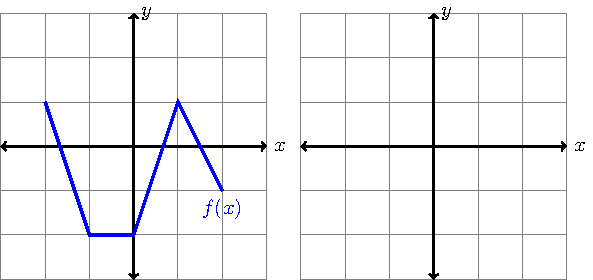
\includegraphics[width=0.65\columnwidth]{figures/0-3-fig2.pdf}
        \end{center}
        \caption{Function transformation for Activity \ref{A:0.3.1}} \label{F:0.3.Act1}
    \end{figure}
\end{activity}
\begin{smallhint}
    \ba
        \item Think of the ``$-$'' in front of $f(x)$ as a $-1$.  What is the difference
            between multiplying by $-1$ and adding $-1$?
        \item Think about the order of mathematical operations.
    \ea
\end{smallhint}
\begin{bighint}
    \ba
        \item $g(x)$ should be a vertical stretch and $h(x)$ should be a vertical shift.
        \item A very methodical way to approach this problem would be to choose several
            particular $x$ values and follow the order of operations to determine the
            output for $k$.
    \ea
\end{bighint}
\begin{activitySolution}
    \ba
        \item The function $g(x)$ should change the sign on all of the $y$ values of $f$.
            The function $h(x)$ will shift all of the $y$ values of $f$ down 1 unit.
        \item The order in which you do the transformations does matter.  In this problem
            the order of operations should be to change the sign on the $y$ value and then
            to shift 1 unit down.
    \ea
    \begin{center}
        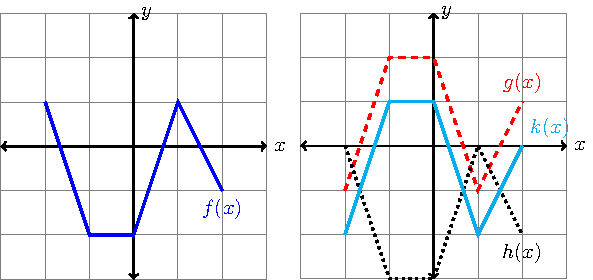
\includegraphics[width=0.65\columnwidth]{figures/0-3-fig2soln.pdf}
    \end{center}
\end{activitySolution}

\aftera




\subsection*{Composition of Functions}
When multiple transformations are applied in sequence, like in Activity \ref{A:0.3.1}, the
resulting function is actually the {\bf composition} of function transformations.  The
concept of a composition encompasses more than just transformations though.  If $f(x)$ and
$g(x)$ are functions where the range of $g(x)$ is a subset of the domain of $f(x)$ we can
form a new function $h(x) = f(g(x))$. This literally means that you are substituting
$g(x)$ in for every instance of the variable $x$ in $f(x)$.  For example, if $f(x) = x^2$
and $g(x) = e^x$ then $h(x) = f(g(x)) = \left( e^x \right)^2$ and $k(x) = g(f(x)) =
e^{(x^2)}$.  

\bex
If $f(x) = x^2$ and $g(x) = x-1$ then find $f(g(3))$, $g(f(3))$, $f(g(x))$, and
$g(f(x))$.
\eex
To evaluate $f(g(3))$ we consider that $g(3) = 2$ and $g(2) = 4$.  Therefore, $f(g(3))=4$.
Similarly, $g(f(3)) = g(9) = 8$.  The function compositions $f(g(x))$ and $g(f(x))$ are
$f(g(x)) = (x-1)^2$ and $g(f(x))=x^2 - 1$.  Notice the difference between these resulting
functions; the order that the composition takes places matters!
\afterex

\subsection*{Symmetry}
There are many ways that a function can be symmetric, but two important symmetries are (1)
reflective symmetry over the $y$-axis, and (2) $180^\circ$ rotational symmetry about the
origin.  A function that has reflective symmetry over the $y$-axis is called an {\bf even
function} and a function with rotational symmetry about the origin is called an {\bf odd
function}.  The reasoning for these names will be evident after completing Activity
\ref{A:0.3.2}.

\begin{activity}\label{A:0.3.2}
    \ba
        \item Based on symmetry alone, is $f(x) = x^2$ an even or an odd function?
        \item Based on symmetry alone, is $g(x) = x^3$ an even or an odd function?
        \item Find $f(-x)$ and $g(-x)$ and make conjectures to complete these sentences:
            \begin{itemize}
                \item If a function $f(x)$ is \underline{even} then $f(-x) =
                    $\underline{\hspace{1in}}.
                \item If a function $f(x)$ is \underline{odd} then $f(-x) =
                    $\underline{\hspace{1in}}.
            \end{itemize}
            Explain why the composition $f(-x)$ is a good test for symmetry of a function.
        \item Classify each of the following functions as even, odd, or neither.
            \[ h(x) = \frac{1}{x}, \quad j(x) = e^x, \quad k(x) = x^2-x^4, \quad n(x) =
            x^3+x^2. \]
        \item For the figure below shows only half of the function $f(x)$.  Draw the left
            half so $f(x)$ is even.  Draw the left half so $f(x)$ is odd. Draw the left
            half so $f(x)$ is neither even nor odd.
            \begin{center}
                \begin{tikzpicture}[scale=0.65]
                    \draw[color=gray] (-3,-3) grid (3,3);
                    \draw[thick, black, <->] (-3,0) -- (3,0) node[anchor=west]{$x$};
                    \draw[thick, black, <->] (0,-3) -- (0,3) node[anchor=west]{$x$};
                    \draw[very thick, blue] (0,0) -- (1,1) -- (2,1) -- (3,-1)
                    node[anchor=north]{$f(x)$}; 
                \end{tikzpicture}
                \begin{tikzpicture}[scale=0.65]
                    \draw[color=gray] (-3,-3) grid (3,3);
                    \draw[thick, black, <->] (-3,0) -- (3,0) node[anchor=west]{$x$};
                    \draw[thick, black, <->] (0,-3) -- (0,3) node[anchor=west]{$x$};
                    \draw[very thick, blue] (0,0) -- (1,1) -- (2,1) -- (3,-1)
                    node[anchor=north]{$f(x)$}; 
                \end{tikzpicture}
                \begin{tikzpicture}[scale=0.65]
                    \draw[color=gray] (-3,-3) grid (3,3);
                    \draw[thick, black, <->] (-3,0) -- (3,0) node[anchor=west]{$x$};
                    \draw[thick, black, <->] (0,-3) -- (0,3) node[anchor=west]{$x$};
                    \draw[very thick, blue] (0,0) -- (1,1) -- (2,1) -- (3,-1)
                    node[anchor=north]{$f(x)$}; 
                \end{tikzpicture}
            \end{center}
    \ea
\end{activity}\aftera


\subsection*{Inverse Functions}
We conclude this section by discussing an important question:  If we know the action of a
function is it possible to undo that action? This question can be rephrased by saying: If
we know the output of a function can we tell exactly what the input was?  The answer to
these questions is that it depends on the type of function.  

Consider, for example, the function $f(x) = x^2$.  If we know that $f(a) = 4$ do we the
value of $a$?  Of course not!  It is obvious that $f(2) = f(-2) = 4$, so just by knowing
the output of the function $f(x) = x^2$ we cannot invert the function and find the input.
What about the function $g(x) = x^3$?  If we know that $g(b) = 8$ then there is only one
unique value of $b$, $b=2$, such that $g(b) = 8$.  Therefore it seems like we can invert
the cubic function.  

The act of {\it reversing the action of a function} can be explored geometrically.
Indeed, in Figure \ref{fig:0.3.inv} we see that if we can simply switch the values of $x$
and $y$ we will get a plot that shows how to undo the action of a function. Geometrically,
switching the role of the $x$ and the $y$ in the function is the same as reflecting over
the line $y=x$.
\begin{figure}[h!]
    \begin{center}
        \begin{tikzpicture}
            \begin{axis}[axis lines=center, xlabel={$x$}, ylabel={$y$}, domain=-4:4,
                ymin=-4, ymax=4, xmin=-4, xmax=4, grid]
                \addplot[smooth, very thick, red, samples=150] {x^3};
                \addplot[smooth, very thick, blue, samples=150] {(x/abs(x))*abs(x)^(1/3)};
                \draw[dashed, thick, fill=black] (axis cs:1.26,2) circle(0.05cm) -- (axis
                cs:2,1.26) circle(0.05cm);
                \draw[dashed, thick, fill=black] (axis cs:-1.26,-2) circle(0.05cm) -- (axis
                cs:-2,-1.26) circle(0.05cm);
                \draw[dashed, thick, fill=black] (axis cs:-0.125,-.5) circle(0.05cm) -- (axis
                cs:-0.5,-0.125) circle(0.05cm);
                \draw[dashed, thick, fill=black] (axis cs:0.125,.5) circle(0.05cm) -- (axis
                cs:0.5,0.125) circle(0.05cm);
                \draw[dashed, thick, fill=black] (axis cs:1.44,3) circle(0.05cm) -- (axis
                cs:3,1.44) circle(0.05cm);
                \draw[dashed, thick, fill=black] (axis cs:-1.44,-3) circle(0.05cm) -- (axis
                cs:-3,-1.44) circle(0.05cm);
                \addplot[smooth, black, dotted, thick] {x};
            \end{axis}
        \end{tikzpicture}
    \end{center}
    \caption{Inverse functions. If $(x,y)$ is on one end of one of the dashed segments,
    then $(y,x)$ is on the other side.}
    \label{fig:0.3.inv}
\end{figure}

The question that remains is when an inverse function actually exists.  This is the same
as asking: ``if I reflect over $y=x$ is the end result a function?''  The answer to this
question is certain ``no'' if the function is $f(x) = x^2$ (as seen in the left-hand plot
of Figure \ref{fig:0.3.inv2}), but if we restrict the domain on $f(x) = x^2$ to $0 \le x < \infty$ then
the result is a function (as seen in the right-hand plot of Figure \ref{fig:0.3.inv2}).
This leads us to the following results:
\begin{itemize}
    \item If a horizontal line passes through a function only once, then it has a unique
        inverse found by interchanging the $x$ and the $y$.
    \item The inverse of a function can be found geometrically by reflecting the graph of
        the function over the line $y=x$.
\end{itemize}
\begin{figure}[ht!]
    \begin{center}
        \begin{tikzpicture}
            \begin{axis}[axis lines=center, xlabel={$x$}, ylabel={$y$}, domain=-2:2,
                ymin=-2, ymax=2, xmin=-2, xmax=2, grid]
                \addplot[smooth, very thick, red, samples=150] {x^2};
                \addplot[smooth, very thick, blue, samples=150] {sqrt(x)};
                \addplot[smooth, very thick, blue, samples=150] {-sqrt(x)};
                \addplot[smooth, black, dotted, thick] {x};
                \draw[black, dashed, thick] (axis cs:1.5,-2) -- (axis cs:1.5,2);
                \draw[fill=black] (axis cs:1.5,1.22) circle(0.07cm);
                \draw[fill=black] (axis cs:1.5,-1.22) circle(0.07cm);
            \end{axis}
        \end{tikzpicture}
        \begin{tikzpicture}
            \begin{axis}[axis lines=center, xlabel={$x$}, ylabel={$y$}, domain=0:2,
                ymin=-2, ymax=2, xmin=-2, xmax=2, grid]
                \addplot[smooth, very thick, red, samples=200] {x^2};
                \addplot[smooth, very thick, blue, samples=200] {sqrt(x)};
                \addplot[smooth, black, dotted, thick] {x};
            \end{axis}
        \end{tikzpicture}
    \end{center}
    \caption{The left-hand plot shows that after reflecting $f(x)=x^2$ across $y=x$ the
    result is not a function.  The right-hand plot shows that under a restriction of the
domain the result can be a function.}
    \label{fig:0.3.inv2}
\end{figure}

\bex
Find the inverse of the following functions.  If necessary, restrict the domain on the
function so that the inverse exists.
\ba
    \item $f(x) = x^2+1$
    \item $g(x) = ax+b$
    \item $h(x) = (2x+8)^3$
\ea
\eex
\ba
    \item To find the inverse of $f(x)$ we first interchange the $x$ and $y$.  Then we
        solve for $y$.  That is:
        \[ \text{Solve for $y$: } x = y^2+1 \quad \implies \quad y = \pm\sqrt{x-1}. \]
        Obviously the resulting solution is two equations.  By convention we choose the
        positive square root and note that the inverse only makes sense if $x\ge 1$.
        Hence, in order for the inverse to make sense we need a restriction on the domain
        of $f(x)$: If $0 \le x < \infty$ then any horizontal line only crosses the  graph
        of $f(x)$ once, and hence the inverse exists and is unique.
        \[ f^{-1}(x) = \sqrt{x-1}, \quad x \ge 1 \]
    \item Interchanging the $x$ and $y$ in this equation gives
        \[ \text{Solve for $y$: } x = ay+b \quad \implies \quad y = \frac{x-b}{a}. \]
        There is no need to restrict the domain of $g(x)$ in this instance since the
        resulting equation is a function.
        \[ g^{-1}(x) = \frac{x-b}{a} = \frac{1}{a} x - \frac{b}{a} \]
    \item Interchanging the $x$ and $y$ in this equation gives
        \[ \text{Solve for $y$: } x = (2y+8)^3 \quad \implies \quad y = \frac{x^{1/3}-8}{2}. \]
        In this instance there is no restriction on the domain of $h(x)$ since (as in part
        (b)) the resulting equation is a function.
        \[ h^{-1}(x) = \frac{x^{1/3}-8}{2} \]
\ea
\afterex

Finally, to tie the ideas of composition and inverses togehter we observe that if the
inverse of a function switches the roles of $x$ and $y$ then the composition
$f^{-1}(f(x))$ should simply give $x$ back.  The logical argument is as follows: 
\[ f \text{ maps } x \text{ to } y \quad \text{ then } \quad f^{-1} \text{ maps } y \text{ to }
    x \]
That is,
\[ f^{-1}(f(x)) = x. \]
Similarly, 
\[ f^{-1} \text{ maps } x \text{ to } y \quad \text{ then } \quad f \text{ maps } y \text{ to }
    x \]
which is written more compactly as
\[ f(f^{-1}(x)) = x. \]
These two equations provide a nice algebraic check when finding inverses.



\begin{summary}
\item A function can be transformed by $F(x) = Af(B(x-C))+D$ where $C$ and $D$ shift the
    function and $A$ and $B$ stretch the function.
\item If $f(-x) = f(x)$ then $f$ is an even function.
\item If $f(-x) = -f(x)$ then $f$ is an odd function.
\item To find the inverse of a function we switch the roles of the $x$ and $y$ variables.
    Geometrically this is the same as reflecting over the line $y=x$.  Occasionally it is
    essential to restrict the domain of the original function in order for the inverse to
    exist.
\item The composition of a function and its inverse is the original input: 
    \[ f(f^{-1}(x)) = x \quad \text{and} \quad f^{-1}(f(x)) = x. \]
\end{summary}


\nin \hrulefill

\begin{exercises} 

\item The functions $f(x)$ and $g(x)$ are defined in the table below.  Use these function
    values to answer the following questions.
    \begin{center}
        \begin{tabular}[h!]{|c||c|c|c|c|c|c|c|}
            \hline
            $x$   & $-3$ &$-2$ &$-1$ &$ 0$ &$ 1$ &$ 2$ & $3$ \\ \hline \hline
            $f(x)$& $ 3$ &$ 1$ &$-1$ &$-3$ &$-1$ &$ 1$ & $3$\\ \hline
            $g(x)$& $-2$ &$-1$ &$ 0$ &$ 1$ &$ 0$ &$ 1$ & $2$\\ \hline
        \end{tabular}
    \end{center}
        (a) $f(-3)$, \quad (b) $g(3)$, \quad (c) $f(g(-3))$, \quad (d) $g(f(3))$, \quad
        (e) $f(g(f(-3)))$ \\
        (f) Write a list of value of $f(-x)$ for $x = -3, -2, \dots, 2, 3$.  Based on
            this list is $f(x)$ an even function, and odd function, or neither?\\
        (g) Repeat part (f) for $g(x)$.
\begin{exerciseSolution}
\end{exerciseSolution}


\item Find the inverse of each of the following functions.  If necessary state a
    restriction on the domain of $f(x)$ so that the inverse actually exists.
    \ba
        \item $f(x) = (2x-3)^2$
        \item $g(x) = x^2 - 2x + 1$
    \ea
\begin{exerciseSolution}
\end{exerciseSolution}


\item The plot on the left shows the function $f(x)$ and the plot on the right shows $g(x)
    = Af(B(x-C))+D$.  Find the appropriate values of $A$, $B$, $C$, and $D$.
    \begin{center}
        \begin{tikzpicture}[scale=\scl]
            \draw[color=gray] (-3,-3) grid (3,3);
            \draw[thick, black, <->] (-3,0) -- (3,0) node[anchor=west]{$x$};
            \draw[thick, black, <->] (0,-3) -- (0,3) node[anchor=west]{$x$};
            \draw[very thick, blue] (-2,2) -- (-1,-1) -- (0,1) -- (1,0) -- (2,1)
            node[anchor=south]{$f(x)$}; 
        \end{tikzpicture} 
        \begin{tikzpicture}[scale=\scl]
            \draw[color=gray] (-3,-3) grid (3,3);
            \draw[thick, black, <->] (-3,0) -- (3,0) node[anchor=west]{$x$};
            \draw[thick, black, <->] (0,-3) -- (0,3) node[anchor=west]{$x$};
            \draw[very thick, red] (-3,0) -- (-2,3) -- (-1,1) -- (0,2) -- (1,1)
            node[anchor=south west]{$g(x)$}; 
        \end{tikzpicture}
    \end{center}
\begin{exerciseSolution}
\end{exerciseSolution}

\item Use the function below to plot \\
    (a) $f(x)-3$, \quad (b) $f(x+1)$, \quad (c) $\frac{1}{2}f(x)$, \quad (d) $-f(x)$,
    \quad and (e) $\frac{1}{f(x)}$. 
    \begin{center}
        \begin{tikzpicture}[scale=\scl]
            \draw[color=gray] (-3,-3) grid (3,3);
            \draw[thick, black, <->] (-3,0) -- (3,0) node[anchor=west]{$x$};
            \draw[thick, black, <->] (0,-3) -- (0,3) node[anchor=west]{$x$};
            \draw[very thick, blue] (-3,1) -- (-2,1) -- (0,0) -- (2,2) -- (3,2)
            node[anchor=south]{$f(x)$}; 
        \end{tikzpicture} 
        \begin{tikzpicture}[scale=\scl]
            \draw[color=gray] (-3,-3) grid (3,3);
            \draw[thick, black, <->] (-3,0) -- (3,0) node[anchor=west]{$x$};
            \draw[thick, black, <->] (0,-3) -- (0,3) node[anchor=west]{$x$};
        \end{tikzpicture}
    \end{center}
\begin{exerciseSolution}
\end{exerciseSolution}


\end{exercises}
\afterexercises



\clearpage

\section{Logarithmic Functions} \label{S:0.4.Logarithms}


\vspace*{-14 pt}
\framebox{\hspace*{3 pt}
\parbox{6.25 in}{\begin{goals}
\item How can we ``undo'' the effects of exponentiation?
\item How can we solve equations involving exponential and logarithmic expressions?
\item What are the properties of logarithmic functions?
\end{goals}} \hspace*{3 pt}}


% \begin{web}
% \item
%     \href{https://www.khanacademy.org/math/algebra2/logarithms-tutorial/logarithm_basics/v/logarithms}{Khan
%     Playlist: Logarithm basics}
% \item
%     \href{https://www.khanacademy.org/math/algebra2/logarithms-tutorial/logarithm_properties}{Khan
%     Playlist: Properties of logarithms}
% \item
%     \href{https://www.khanacademy.org/math/algebra2/logarithms-tutorial/natural_logarithm}{Khan
%     Playlist: Natural logarithms}
% \item
%     \href{https://www.khanacademy.org/math/algebra2/exponential_and_logarithmic_func/logarithmic-equations/v/solving-logarithmic-equations_dup_1}{Khan
%     Playlist: Solving logarithmic equations}
% \end{web}

\nin \hrulefill


\subsection*{Introduction}

In section \ref{S:0.2.Exponentials} we studied exponential functions to model a
variety of different settings.  It is straightforward to verify that the graph of an
exponential function passes the ``horizontal line test'' described in section
\ref{S:0.3.Transformations}, and so we should expect exponential functions to have
corresponding inverse functions.  In this section we will define the \emph{logarithm} to
be the inverse function for an exponential.

\begin{pa} \label{PA:0.4}
	Carbon-14 ($^{14}$C) is a radioactive isotope of carbon that occurs naturally in the Earth's atmosphere.  During photosynthesis, plants take in $^{14}$C along with other carbon 	isotopes, and the levels of  $^{14}$C in living plants are roughly the same as atmospheric levels.  Once a plant dies, it no longer takes in any additional  $^{14}$C.  Since  $^{14}$C in the dead plant decays at a predictable rate (the half-life of $^{14}$C is approximately 5,730 years), we can measure  $^{14}$C levels in dead plant matter to get an estimate on how long ago the plant 	died.
	Suppose that a plant has 0.02 milligrams of $^{14}$C when it dies.
\ba
	\item Write a function that represents the amount of $^{14}$C remaining in the plant after $t$ years.
	\item Complete the table for the amount of $^{14}$C remaining $t$ years after the death of the plant.
        \begin{center}
            \begin{tabular}[h!]{| l |c|c|c|c|c|c|c|c|}
                \hline
                t & 0 & 1 & 5 & 10 & 100 & 1000 & 2000 & 5730 \\ \hline
                $^{14}$C Level & 0.02 & & & & & & & \\ \hline
            \end{tabular}
        \end{center}
	\item Suppose our plant died sometime in the past.  If we find that there are 0.014 milligrams of $^{14}$C present in the plant now, estimate the age of the plant to within 50 years.
        \ea
\end{pa} \afterpa


\subsection*{Logarithms}

\begin{definition}[logarithm]
Let $b>0$ with $b\neq1$. The logarithm of $x$ with base $b$ is defined by
	\[
		\log_{b}x=y\qquad\mbox{if and only if}\qquad x=b^{y}.
	\]
The expression $\log_{b}x$ represents the power to which $b$ needs to be raised in order to get $x$.

Two frequently used logarithmic functions are $\log_{10}x$ (frequently written $\log x$) and the natural logarithm $\log_{e}x$ (frequently written $\ln x$).
\end{definition}

Note that we have specifically defined logarithms to be inverse functions for
exponentials. For instance, $\log_{10}{1000} = 3$, since $10^{3} = 1000$.  Logarithmic
functions give us a way to re-write exponential expressions and, more importantly, solve
equations involving variables in an exponent.

\subsection*{Properties of Logarithms}
Since logarithms and exponentials are inverse functions, many of the properties of
logarithmic functions can be deduced directly from the properties of exponential
functions.  For example, the domain of all logarithmic functions is $(0,\infty)$ and the
range of all logarithmic functions is $(-\infty,\infty)$ because those are the range and
domain, respectively, of exponential functions.  Similarly, logarithmic functions have a
vertical asymptote at $x = 0$ because exponential functions have a horizontal asymptote at
$y = 0$. These features can be seen in Figure \ref{F:0.4.Ex1}. 

\begin{figure}[ht!]     
	\begin{center}         
% 		\begin{tikzpicture}[scale=1]             
% 			\begin{axis}[axis lines=center, xlabel={$x$}, ylabel={$y$}, domain=-2:4,
% 							ymin=-3, ymax=3,xmin=-2,xmax=4]
% 				\addplot[smooth, thick, blue, samples=150] {ln(x)}
% 						[below right] node[pos=0.75] {\color{blue}$y=\ln{x}$};
% 				\addplot[smooth, thick, red, samples=150] {exp(x)}
% 						[above left] node[pos=0.02] {\color{red}$y=e^{x}$};
% 				\addplot[smooth, black, dotted, thick] {x}
% 						[below right] node[pos=0.7] {\color{black}$y=x$};
% 			\end{axis}
% 		\end{tikzpicture}     
        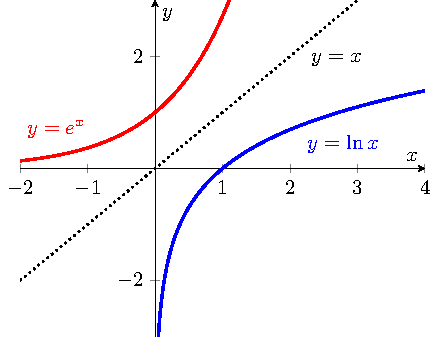
\includegraphics[width=0.5\columnwidth]{figures/0-4-fig1.pdf}
	\end{center}     
\caption{Graphs of the functions $y=e^{x}$ and $y=\ln{x}$.}     
\label{F:0.4.Ex1} 
\end{figure}

The following properties of logarithms can be deduced from the properties of exponential functions and the definition of the logarithm.  These properties are especially useful in simplifying or solving logarithmic and exponential equations.
\begin{theorem}[Properties of Logarithms]
For $b>0$, $b \ne 1$, and $x,y>0$:
\begin{enumerate}
\item $\log_{b}1=0$ \quad (which is the same as the exponent rule $b^0 = 1$)
\item $\log_{b}b=1$ \quad (which is the same as the exponent rule $b^1 = b$)
\item $\log_{b}\left(xy\right)=\log_{b}x+\log_{b}y$ \quad (which is the same as the
    exponent rule $b^{m+n} = b^mb^n$)
\item $\log_{b}\left(\dfrac{x}{y}\right)=\log_{b}x-\log_{b}y$ \quad (which is the same as the
    exponent rule $b^{m-n} = \frac{b^m}{b^n}$)
\item $\log_{b}x^{r}=r\,\log_{b}x$ \quad (which is the same as the exponent rule $(b^m)^n
    = b^{mn}$)
\item $\log_{b}b^{x}=x$
\item $b^{\log_{b}x}=x$
\item $\log_{b}x=\log_{b}y$ if and only if $x=y$
\item $\log_a b = \frac{\log_c a}{\log_c b}$ \quad (this is called the change of base formula)
\end{enumerate}
\end{theorem}

Euler's number, $e$, shows up so often that we give a special name to the associated
logarithm.  The logarithm $\log_e (x)$ is called the natural logarithm and is written as
$\ln(x)$.  We will see later in this course that the exponential function $f(x) = e^x$ has
very special calculus properties and as such the natural logarithm has very special
properties as well.  With this in mind, most mathematicians and scientists use $e^x$ and
$\ln(x)$ as their preferred exponential and logarithmic functions.


\begin{activity}\label{A:0.4.1}
    Use the definition of a logarithm along with the properties of logarithms to answer
    the following.
    \ba
\item Write the exponential expression $8^{1/3} = 2$ as a logarithmic expression.
\item Write the logarithmic expression $\log_2 \frac{1}{32} = -5$ as an exponential
    expression.
\item What value of $x$ solves the equation $\log_2 x = 3$?
\item What value of $x$ solves the equation $\log_2 4 = x$?
\item Use the laws of logarithms to rewrite the expression $\log \left( x^3 y^5 \right)$
    in a form with no logarithms of products, quotients, or powers.
\item Use the laws of logarithms to rewrite the expression $\log \left( \frac{x^{15}
    y^{20}}{z^4} \right)$
    in a form with no logarithms of products, quotients, or powers.
\item Rewrite the expression $\ln(8) + 5 \ln(x) + 15 \ln(x^2+8)$ as a single logarithm.
    \ea


\end{activity}
\begin{smallhint}
    Use the properties of logarithms.
\end{smallhint}
\begin{bighint}
    Use the properties of logarithms.
\end{bighint}
\begin{activitySolution}
    \ba
\item $8^{1/3} = 2$ is equivalent to $\log_8 2 = \frac{1}{3}$.
\item $\log_2 \frac{1}{32} = -5$ is equivalent to $2^{-5} = \frac{1}{32}$.
\item $\log_2 x = 3$ is equivalent to $x = 2^3 = 8$.
\item $\log_2 4 = x$ is equivalent to $2^x = 4$ and we see that $x=2$ since $2^2 = 4$.
\item Using the product and power properties
    \[ \log\left( x^3 y^5 \right) = 3\log(x) + 5\log(y). \]
\item Using the product, power, and quotient properties
    \[ \log\left( \frac{x^{15} y^{20}}{z^4} \right) = 15\log(x) + 20\log(y) - 4\log(z). \]
\item Using the power and product properties
    \[ \ln(8) + 5 \ln(x) + 15\ln(x^2+8) = \ln\left( 8 x^5 \left( x^2 + 8 \right)^{15}
        \right) \]
    \ea
\end{activitySolution}

\aftera



\bex
Find a value of $x$ for which $3^{x}=13$.
\eex
To isolate the variable $x$, we should take the logarithm of both sides. For convenience,
let's choose to use the natural logarithm.
	\[
		\ln(3^{x})=\ln(13).
	\]
Applying logarithm property (5), we find
	\[
		x\,\ln 3=\ln 13.
	\]
Solving algebraically for $x$ yields
	\[
		x=\frac{\ln 13}{\ln 3}\approx2.3347.
	\]
NOTE: Our choice to use the natural logarithm was arbitrary. We could have chosen any base
for our logarithm to solve this equation.
% \afterex

\bex
In 1970, the population of the United States was approximately 205.1 million people. Since
that time, the population has grown at a continuous growth rate of approximately 1.05\%. Assuming that this growth rate continues, when would we expect the population of the United States to reach 350 million?
\eex
Since the rate of growth of the population is proportional to the size of the population, we should use an exponential model for this problem. That is, we want
	\[
		P(t)=P_{0}e^{rt}
	\]
where $t$ is the number of years after 1970, $P(t)$ is the population (in millions) of the
United States at time $t$, $P_{0}$ is the population (in millions) of the United States in
1970 (i.e. $t=0$) and $r$ is the continuous rate of growth of the population. To determine when the population will reach 350 million, we must solve the equation 
	\[
		350=205.1e^{0.0105t}.
	\]
To solve for $t$, we need to first solve for the exponential expression by itself and then use logarithms. Dividing both sides of the equation by 205.1 gives
	\[
		\frac{350}{205.1}=e^{0.0105t}.
	\]
Taking the natural logarithm of both sides gives
	\[
		\ln\left(\frac{350}{205.1}\right)=\ln\left(e^{0.0105t}\right).
	\]
Applying logarithm property (6), we find
	\[
		\ln\left(\frac{350}{205.1}\right)=0.0105t.
	\]
Finally, solving algebraically for $t$ gives
	\[
		t=\frac{1}{0.0105}\ln\left(\frac{350}{205.1}\right)\approx50.9\,\mbox{years}.
	\]
Thus, we expect the population of the United States to reach 350 million in 2021 (approximately 51 years after 1970).
\afterex

\begin{activity}\label{A:0.4.2}
    Solve each of the following equations for $t$, and verify your answers using a calculator.
	\ba
		\item $\ln t=4$
		\item $\ln(t+3)=4$
		\item $\ln(t+3)=\ln4$
		\item $\ln(t+3)+\ln(t)=\ln4$
		\item $e^{t}=4$
		\item $e^{t+3}=4$
		\item $2e^{t+3}=4$
		\item $2e^{3t+2}=3e^{t-1}$
	\ea

\end{activity}
\begin{smallhint}
    
\end{smallhint}
\begin{bighint}
    
\end{bighint}
\begin{activitySolution}
    \ba
        \item $t = e^4$
        \item $t+3 = e^4$ so $t = e^4 - 3$
        \item $t+3 = 4$ so $t=1$
        \item Using the product property for logarithms, $\ln(t(t+3)) = \ln(4)$ so $t^2 +
            3t = 4$.  This is quadratic so we rearrange to get $t^2 + 3t - 4 = 0$ which
            factors to $(t+4)(t-1) = 0$ so the solutions are $t=1$ and $t=-4$.
            Substituting back to the original equation we see that $\ln(-4+3)$ and
            $\ln(-4)$ do not exist so the only solution is $t=1$.
        \item $t=\ln(4)$
        \item $t= \ln(4) = 3$
        \item $t+3 = \ln(2)$ so $t = \ln(2) = 3$
        \item For the final problem we first divide by $2$ and take the natural logarithm
            of both sides.
            \[ e^{3t+1} = \frac{3}{2} e^{t-1} \implies 3t+1 = \ln(3/2) + t-1. \]
            Therefore, $2t = \ln(3/2) - 2$ so $t=\frac{1}{2} \left( \ln(3/2) - 2 \right)$.
    \ea
\end{activitySolution}
\aftera

\begin{activity}\label{A:0.4.3}
    Consider the following equation:
	\[
		7^{x} = 24
	\]

	\ba
		\item How many solutions should we expect to find for this equation?
		\item Solve the equation using the log base 7.
		\item Solve the equation using the log base 10.
		\item Solve the equation using the natural log.
		\item Most calculators have buttons for $\log_{10}$ and $\ln$, but none have a button for $\log_{7}$. Use your previous answers to write a formula for $\log_{7}x$ in terms of 					$\log x$ or $\ln x$.
	\ea

\end{activity}
\begin{smallhint}
   Use the properties of logarithms and exponential functions. 
\end{smallhint}
\begin{bighint}
   Use the properties of logarithms and exponential functions. 
\end{bighint}
\begin{activitySolution}
   \ba
    \item We expect 1 solution since the exponential function $7^x$ is always increasing.
    \item $\log_7 (24) = x$.
    \item $\log (7^x) = \log(24)$ so $x\log(7) = \log(24)$ and therefore $x =
        \frac{\log(24)}{\log(7)}$
    \item $\ln (7^x) = \ln(24)$ so $x\ln(7) = \ln(24)$ and therefore $x =
        \frac{\ln(24)}{\ln(7)}$
    \item $\log_7(x) = \frac{\ln(x)}{\ln(7)} = \frac{\log(x)}{\log(7)}$.
   \ea
\end{activitySolution}

\aftera

\begin{activity}\label{A:0.4.4}
\ba
\item In the presence of sufficient resources the population of a colony of bacteria exhibits exponential growth, doubling once every three hours. What is the corresponding continuous (percentage) growth rate?
\item A hot bowl of soup is served at a dinner party.  It starts to cool according to
    Newton's Law of Cooling so its temperature, $T$ (measured in degrees Fahrenheit) after
    $t$ minutes is given by
    \[ T(t) = 65 + 186 e^{-0.06t}. \]
    How long will it take from the time the food is served until the temperature is
    $120^\circ$F?
\item The velocity (in ft/sec) of a sky diver $t$ seconds after jumping is given by 
    \[ v(t) = 80\left( 1-e^{-0.2t} \right). \]
    After how many seconds is the velocity 75 ft/sec?
\ea
\end{activity}
\begin{smallhint}
    Use the properties of logarithms.
\end{smallhint}
\begin{bighint}
    Use the properties of logarithms.
\end{bighint}
\begin{activitySolution}
    \ba
        \item If the population doubles every three hours then the exponential function
            describing the growth is $P(t) = P_0 2^{t/3}$.  We want to find the continuous
            growth rate so we want to write the function as $P(t) = P_0 e^{kt}$.
            Therefore we need to solve the equation $2^{t/3} = e^{kt}$ for $k$.  Taking
            the natural logarithm of both sides gives
            $\ln \left( 2^{t/3} \right) = kt$, and using the rules of exponents we see
            that $\frac{t}{3} \ln(2) = kt$.  Subtracting $kt$ from both sides and
            factoring the $t$ gives $t\left( \frac{\ln(2)}{3} - k \right) = 0$ so we
            immediately see that $k = \ln(2)/3$.
        \item We need to solve the equation $65+186e^{-0.06t} = 120$.  Subtracting 65 and
            dividing by 186 gives $e^{-0.06t} = \frac{55}{186}$.  Taking the natural
            logarithm of both sides and then dividing by -0.06 gives $t =
            -\frac{1}{0.06} \ln \left( \frac{55}{186} \right)$.
        \item We need to solve the equation $80\left( 1-e^{-0.2t} \right) = 75$.  Dividing
            by 80 gives $1-e^{-0.2t} = \frac{15}{16}$.  Hence, $e^{-0.2t} =
            \frac{1}{16}$ and taking the natural logarithm of both sides gives $-0.2t =
            \ln(1/16)$.  Therefore, $t = -\frac{1}{0.2} \ln\left( \frac{1}{16} \right)$.
    \ea
\end{activitySolution}

\aftera


\begin{summary}
\item A logarithmic function can be written in the form $f(x)=\log_{b}x$ where $b>0$, $b\ne1$, and $x>0$.
\item Logarithmic functions are defined to be inverse functions for exponentials.  That is
	\[
		\log_{b}x=y\qquad\mbox{if and only if}\qquad x=b^{y}.
	\]
\item Solving equations that contain exponential expressions frequently requires the use of logarithms; solving equations that contain logarithmic expressions frequently requires the use of exponentials.
\end{summary}

% exercises go here
\begin{exercises} 

\item 
\begin{exerciseSolution}
\end{exerciseSolution}



\end{exercises}
\afterexercises





\clearpage

% \section{Trigonometric Functions} \label{S.0.5.TrigFunctions}


\vspace*{-14 pt}
\framebox{\hspace*{3 pt}
\parbox{6.25 in}{\begin{goals}
\item  How can we model systems that vary in a smooth, wavelike cycle, rising and falling again and again?  
\item How can we model the shape of waves in water, sound waves, radio waves, the motion of the tides in and out over the course of a day, the shaking of an earthquake, or the varying time of sunrise over the course of a year?
\end{goals}} \hspace*{3 pt}}


\begin{web}
\item
    \href{https://www.khanacademy.org/math/trigonometry/unit-circle-trig-func/radians_tutorial/v/introduction-to-radians}{Khan
    Playlist: Radian measure and arc length}
\item
    \href{https://www.khanacademy.org/math/trigonometry/unit-circle-trig-func/Trig-unit-circle}{Khan
    Playlist: Trig on the unit circle}
\item
    \href{https://www.khanacademy.org/math/trigonometry/unit-circle-trig-func/trig-functions-special-angles}{Khan
    Playlist: Trig functions of special angles}
\item
    \href{https://www.khanacademy.org/math/trigonometry/unit-circle-trig-func/inverse_trig_functions}{Khan
    Playlist: Inverse trig functions}
\item
    \href{https://www.khanacademy.org/math/trigonometry/trig-function-graphs/trig_graphs_tutorial/v/midline-amplitude-period}{Khan
    Playlist: Graphs of trig functions}
\item
    \href{https://www.khanacademy.org/math/trigonometry/trig-function-graphs/modeling-periodic-functions}{Khan
    Playlist: Modeling with periodic functions}
\end{web}

\nin \hrulefill


\subsection*{Introduction}

You probably first learned about sines, cosines, and tangents when you were studying triangles.  However, these functions are amazingly useful in an enormous variety of contexts.  These functions are so handy that scientists and mathematicians always keep them in mind as part of our standard toolbox.  We use sines and cosines whenever we see anything that varies in a smooth wave cycle, going up and down by the same amount, again and again on a regular basis.

% Your preview activity goes here

\begin{pa} \label{PA:0.5}
A tall water tower is swaying back and forth in the wind.  Using an ultrasonic ranging
device, we measure the distance from our device to the tower (in centimeters) every two
seconds with these measurements recorded below.  

\medskip

\begin{tabular}{| c | c | c | c | c | c | c | c | c | c | c | c |}
\hline
Time (sec) & 0 & 2 & 4 & 6 & 8 & 10 & 12 & 14 & 16 & 18 & 20 \\
\hline
Distance (cm) & 30.9 & 23.1 & 14.7 & 12.3 & 17.7 & 26.7 & 32.3 & 30.1 & 21.8 & 13.9 & 12.6 \\
\hline
\end{tabular}

% \begin{enumerate}
\ba
\item Use the coordinate plane below to create a graph of these data points.
    \begin{center}
        \begin{tikzpicture}
            \begin{axis}[axis lines=center, xmin=-0.5, xmax=20, ymin=0, ymax=40,
                xtick={2,4,6,8,10,12,14,16,18,20}, ytick={5,10,15,20,25,30,35,40}, grid,
            xlabel={Time (sec)}, ylabel={Distance (cm)}]
                \addplot[smooth] {0*x};
            \end{axis}
        \end{tikzpicture}
    \end{center}
\item What is the water tower's maximum distance away from the device? % 32.3 cm
\item What is the smallest distance measured from the tower to the device? % 12.3 cm
\item If the water tower was sitting still and no wind was blowing, what would be the distance from the tower to the device?  We call this the tower's equilibrium position.% About 22.3 cm
\item What is the maximum distance that the tower moves away from its equilibrium position?  We call this the amplitude of the oscillations.  % About 10 centimeters
\item How much time does it take the water tower to sway back and forth in a complete cycle?  We call this the period of oscillation.  % About 14 seconds
% \end{enumerate}



\ea
\end{pa} \afterpa



\subsection*{Measuring Angles with Radians}

Sines, cosines, and tangents are very useful when studying triangles.  The input into each
of these functions is an angle, and the output tells us the ratio of the lengths of the
sides of the triangle.  There are two commonly used units for measuring angles, degrees
and radians, and so there are two commonly used versions of the trigonometric functions.
There's $\sin x$ where $x$ is in degrees, and there's $\sin x$ where $x$ is in radians.
Calculus is a lot easier if we measure angles in radians, so that's what we'll use
throughout this course.  If you ever have trouble getting the right numbers from your
calculator, you may want to double check that your calculator is in radian mode.

So, what is a radian?  

\begin{definition}
    A {\bf radian} is a measure of angle which is defined so that if we have an angle with
    a size of one radian on a unit circle (with a radius $r= 1$), then the length of the
    arc along the circumference of the circle is also equal to one, as we see in Figure
    \ref{fig:0.5.radian}.  Because the circumference of a circle is $2 \pi r$, this means
    that for one complete circle, 
    \[ 360^\circ = 2 \pi \text{ radians.} \]
    Similarly half a circle is
    \[ 180^\circ = \pi \text{ radians} \]
    and a right angle is 
    \[ 90^\circ = \frac{\pi}{2} \text{ radians.} \]  
    So one radian is 
    \[ 57.3^\circ \approx \frac{180^\circ}{\pi} = 1 \text{ radian}. \]
\end{definition}

% \resizebox{3in}{!}{
% \begin{picture}(80,80)(10,10)
% \thicklines
% \put(50,50){\circle{40}}
% \put(70,50){\circle*{3}}
% \put(20,50){\line(1,0){60}}
% \put(50,20){\line(0,1){60}}
% \put(50,50){\line(2,3){13}}
% \qbezier(56,50)(57,54)(54,56)
% \end{picture}}
% \begin{picture}(80,80)(60,10)
% \put(0,140){Arc Length = 1}
% \put(-32,125){\resizebox{1cm}{!}{1 radian}}
% \put(-44,105){\footnotesize radius = 1}
% \end{picture}
% 

\begin{figure}[h!]
    \centering
    \begin{tikzpicture}[scale=1.5]
        \draw[<->, very thick] (-1.5,0) -- (1.5,0) node[anchor=west]{$x$}; 
        \draw[<->, very thick] (0,-1.5) -- (0,1.5) node[anchor=south]{$y$}; 
        \draw (0.5,0) node[anchor=north]{$1$};
        \draw[thick, color=blue] (0,0) circle(1cm);
        \draw[color=black, fill=black] (1,0) circle(0.035cm) node[anchor=south west]{0 radians
        $=0^\circ$};
        \draw[color=black, fill=black] (1,0) circle(0.035cm) node[anchor=north west]{$2 \pi$ radians
        $=360^\circ$};
        \draw[color=black, fill=black] (0,1) circle(0.035cm) node[anchor=south
        west]{$\pi/2$ radians $=90^\circ$};
        \draw[color=black, fill=black] (-1,0) circle(0.035cm) node[anchor=south
        east]{$\pi$ radians $=180^\circ$};
        \draw[color=black, fill=black] (0,-1) circle(0.035cm) node[anchor=north
        east]{$3\pi/2$ radians $=270^\circ$};
    \end{tikzpicture}
    \begin{tikzpicture}[scale=1.5]
        \draw[<->, very thick] (-1.5,0) -- (1.5,0) node[anchor=west]{$x$}; 
        \draw[<->, very thick] (0,-1.5) -- (0,1.5) node[anchor=south]{$y$}; 
        \draw (0.5,0) node[anchor=north]{$1$};
        \draw[thick, color=blue] (0,0) circle(1cm);
        \draw[color=black, very thick] (0,0) -- (0.54,0.84);
        \draw[color=black, fill=black] (0.54,0.84) circle(0.035cm) node[anchor=south
        west]{1 radian $\approx 57.3^\circ$};
        \draw[color=black, very thick] (1,0) arc(0:57.3:1cm);
        \draw[black] (0.92,0.4) node[anchor=west]{Arc Length = 1};
    \end{tikzpicture}
    \caption{Common radian measures.}
    \label{fig:0.5.radian}
\end{figure}

Because we define the radian in this way, this means that the arc length $s$ along the
circumference of a circle with radius $r$ over angle $\theta$ can be calculated as
\[ s = r \theta \]
as long as the angle $\theta$ is measured in radians.

\begin{center}
    \begin{tikzpicture}[scale=1]
        \draw[thick, color=blue] (0,0) circle(1.5cm);
        \draw[color=black, very thick] (0,0) -- (0.61,1.37) arc(66:-23:1.5cm) -- (0,0);
        \draw (0,0.1) node[anchor=west]{$\theta$};
        \draw (1.4,0.2) node[anchor=south west]{$s$};
        \draw (0.8,-0.3) node[anchor=north]{$r$};
    \end{tikzpicture}
\end{center}


\subsection*{Sine and Cosine on the Unit Circle}

Let's draw a unit circle with its center at the origin and think about a point moving along the circumference of this circle.  We start with the point on the $x$ axis with coordinates (1,0), as shown in the figure below, and define this location to be an angle of $\theta = 0$ radians.  Then, we let this point move up, so that our point is at an angle $\theta$ above the $x$ axis.  The sine and cosine functions are defined so that they give us the coordinates of our point:   
\[ x = \cos \theta \quad \text{and} \quad y = \sin \theta \]


\begin{center}
    \begin{tikzpicture}[scale=1.5]
        \draw[<->, very thick] (-1.5,0) -- (1.5,0) node[anchor=west]{$x$}; 
        \draw[<->, very thick] (0,-1.5) -- (0,1.5) node[anchor=south]{$y$}; 
        \draw[thick, color=blue] (0,0) circle(1cm);
        \draw[color=black, very thick] (0,0) -- (0.54,0.84);
        \draw[color=black,fill=black] (0.54,0.84) circle(0.04cm)
        node[anchor=south west]{$(x,y)=(\cos\theta,\,\sin\theta)$};
        \draw[->, thick] (0,0) -- (0.54,0);
        \draw[->, thick] (0.54,0) -- (0.54,0.84);
        \draw (0.26,0) node[anchor=north]{$x$};
        \draw (0.54,0.42) node[anchor=west]{$y$};
        \draw[color=black, fill=black] (1,0) circle(0.035cm) node[anchor=south
        west]{$(1,0)$};
    \end{tikzpicture}
\end{center}

% \resizebox{4in}{!}{
% \begin{picture}(200,100)(0,0)
% \thicklines
% \put(50,50){\circle{40}}
% \put(70,50){\circle*{3}}
% \put(20,50){\line(1,0){60}}
% \put(50,20){\line(0,1){60}}
% \put(73,52){\tiny(1,0)}
% \put(130,50){\circle{40}}
% \put(143,65){\circle*{3}}
% \put(100,50){\line(1,0){60}}
% \put(130,20){\line(0,1){60}}
% \put(130,50){\line(5,6){13}}
% \put(144,67){\tiny$(x,y)=(\cos \theta, \sin \theta)$}
% \put(134,51){\tiny$\theta$}
% \put(143,50){\vector(0,1){14} }
% \put(144,53){\tiny$y$}
% \put(130,47){\vector(1,0){12} }
% \put(134,42){\tiny$x$}
% \end{picture}}

This means that an angle of $\theta = 2 \pi$ carries us around one full circle and brings
us back to our starting point on the $x$ axis again, with coordinates (1,0).  That means
that $\sin 2 \pi = \sin 0 = 0$.  Similarly $\theta = 4 \pi$ carries us around two full
circles, and $\theta = 6 \pi$ carries us around three full circles. 

Next we can use the Pythagorean Theorem, and remember that our hypotenuse is equal to one to see that
\[ \sin^2 \theta + \cos^2 \theta = 1 \]
This is a very useful relationship!


\subsection*{Sine and Cosine as Functions} 

To get beyond trigonometry, rather than using the angle $\theta$ as the input to our sine
and cosine functions, instead we will put our function input on the $x$ axis.  Then we can
plot the output of on the $y$ axis.  This produces the following graph:
\begin{center}
    \begin{tikzpicture}
        \begin{axis}[axis lines=center, xlabel={$x$}, xmin=-7, xmax=7,
                ymin=-1.5, ymax=1.5, ytick={-1,1}, xtick={-6.28, -4.71, -3.14, -1.57,
                1.57, 3.14, 4.71, 6.28},
            xticklabels={$-2\pi$,$-\frac{3}{2}\pi$,$-\pi$,$-\frac{1}{2}\pi$,$\frac{1}{2}\pi$,$\pi$,$\frac{3}{2}\pi$,$2\pi$},
        grid, xscale=2]
            \addplot[smooth, very thick, color=blue, domain=-6.5:6.5, samples=100] {sin(deg(x))};
            \draw (axis cs:0,1) node[anchor=south west]{$y = \sin(x)$};
        \end{axis}
    \end{tikzpicture}
\end{center}

% \resizebox{4in}{!}{\includegraphics{0-5-TrigonometricFunctions2.jpg}}

\noindent
Here we can see that the range (output) of the sine function is the interval from $-1$ to $+1$.  ($\sin x$ can never equal 2!)  The domain (input) of the sine function is extends from $-\infty$ to $+\infty$, but the cycle repeats every $2 \pi$ along the $x$ axis.  (Do you understand how the definition of sine on the unit circle makes both of these facts true?)

The following terms will be very important when we describe functions like this:

\begin{itemize}
\item The \emph{period} of a function is how far along the $x$ axis it takes to complete one full cycle.
\item The \emph{amplitude} of a function is how far it goes on the $y$ axis above and below its average value.
\end{itemize}
The function $f(x) = \sin x$ has a period of $2 \pi$ and an amplitude of $1$.  If we plot
both the sine and the cosine functions together we see the following graph:
\begin{center}
    \begin{tikzpicture}
        \begin{axis}[axis lines=center, xlabel={$x$}, ylabel={$y$}, xmin=0, xmax=7,
                ymin=-1.25, ymax=1.25, ytick={-1,-0.5,0.5,1}, xtick={0.785,
                1.57, 2.356, 3.14, 3.927, 4.71, 5.498, 6.28},
                xticklabels={$\frac{1}{4}\pi$,$\frac{1}{2}\pi$, $\frac{3}{4}\pi$,$\pi$,
                $\frac{5}{4}\pi$,$\frac{3}{2}\pi$,$\frac{7}{4}\pi$,$2\pi$},
                yticklabels={$-1$,$-\frac{1}{2}$,$\frac{1}{2}$,$1$},
        grid, xscale=2]
            \addplot[smooth, very thick, color=blue, domain=0:6.5, samples=100] {sin(deg(x))};
            \addplot[smooth, dashed, very thick, color=red, domain=0:6.5, samples=100]
            {cos(deg(x))};
            \draw (axis cs:2.4,0.7) node[anchor=south west]{$y = \sin(x)$};
            \draw (axis cs:5.5,0.7) node[anchor=south east]{$y = \cos(x)$};
        \end{axis}
    \end{tikzpicture}
\end{center}
% \resizebox{4in}{!}{\includegraphics{0-5-TrigonometricFunctions1.jpg}}
From this we see that the function $g(x) = \cos x$ also has a period of $2 \pi$ and an
amplitude of $1$.  The difference is that $\sin 0 = 0$, so the sine function starts at its
average value, halfway between a peak and a trough.  On the other hand $\cos 0 = 1$, so
the cosine function starts at a peak.  This means that we can turn a cosine function into
a sine function and visa versa simply by shifting:
\[ \sin(x) = \cos \left( x - \frac{\pi}{2} \right) \quad \text{and} \quad \cos(x) = \sin
\left( x + \frac{\pi}{2} \right). \]


\subsection*{Sinusoidal Functions in the Real World}

To model real data with the sine function, we must be able to change the amplitude, the
period, and the average value of our wave, to get what we call a \emph{sinusoidal}
function.  Every sinusoidal function can be written either of these two forms:

\begin{callout}
    \[ f(t) = A \sin( B ( t - t_0) ) + C \mbox{ or } f(t) = A \sin( B t + \phi) + C \]

\begin{itemize}
\item $A$ is the amplitude.  
\item $B$ is the angular frequency, which determines the period, with $B = \frac{2 \pi}{\mbox{Period}}$.  
\item $C$ is the average value.  
\item $t_0$ is the shift along the $t$ axis, a time when $f$ is at an average value and increasing
\item $\phi$ is the shift in radians, the angle at which the oscillations begin
\end{itemize}
\end{callout}

The parameter $B$ can be a little surprising.  Because $B$ is inversely related to the
period, this means that larger values of $B$ result in a shorter period, and smaller
values of $B$ result in a longer period, as we see in the graphs below:
\def\scl{0.89}
\begin{center}
    \begin{tikzpicture}[scale=\scl]
        \begin{axis}[axis lines=center, xmin=0, xmax=6.28, ymin=-1.25, ymax=1.25,
            domain=0:6.28, xlabel={$t$}, title={$\sin(t)$}, grid, xtick={0.785,
                1.57, 2.356, 3.14, 3.927, 4.71, 5.498, 6.28},
                xticklabels={$\frac{1}{4}\pi$,$\frac{1}{2}\pi$, $\frac{3}{4}\pi$,$\pi$,
                $\frac{5}{4}\pi$,$\frac{3}{2}\pi$,$\frac{7}{4}\pi$,$2\pi$}]
            \addplot[smooth, color=blue, very thick, samples=100] {sin(1*deg(x))};
        \end{axis}
    \end{tikzpicture}
    \begin{tikzpicture}[scale=\scl]
        \begin{axis}[axis lines=center, xmin=0, xmax=6.28, ymin=-1.25, ymax=1.25,
            domain=0:6.28, xlabel={$t$}, title={$\sin(2t)$}, grid, xtick={0.785,
                1.57, 2.356, 3.14, 3.927, 4.71, 5.498, 6.28},
                xticklabels={$\frac{1}{4}\pi$,$\frac{1}{2}\pi$, $\frac{3}{4}\pi$,$\pi$,
                $\frac{5}{4}\pi$,$\frac{3}{2}\pi$,$\frac{7}{4}\pi$,$2\pi$}]
            \addplot[smooth, color=blue, very thick, samples=100] {sin(2*deg(x))};
        \end{axis}
    \end{tikzpicture}
    \begin{tikzpicture}[scale=\scl]
        \begin{axis}[axis lines=center, xmin=0, xmax=6.28, ymin=-1.25, ymax=1.25,
            domain=0:6.28, xlabel={$t$}, title={$\sin(3t)$}, grid, xtick={0.785,
                1.57, 2.356, 3.14, 3.927, 4.71, 5.498, 6.28},
                xticklabels={$\frac{1}{4}\pi$,$\frac{1}{2}\pi$, $\frac{3}{4}\pi$,$\pi$,
                $\frac{5}{4}\pi$,$\frac{3}{2}\pi$,$\frac{7}{4}\pi$,$2\pi$}]
            \addplot[smooth, color=blue, very thick, samples=100] {sin(3*deg(x))};
        \end{axis}
    \end{tikzpicture}
    \begin{tikzpicture}[scale=\scl]
        \begin{axis}[axis lines=center, xmin=0, xmax=6.28, ymin=-1.25, ymax=1.25,
            domain=0:6.28, xlabel={$t$}, title={$\sin(4t)$}, grid, xtick={0.785,
                1.57, 2.356, 3.14, 3.927, 4.71, 5.498, 6.28},
                xticklabels={$\frac{1}{4}\pi$,$\frac{1}{2}\pi$, $\frac{3}{4}\pi$,$\pi$,
                $\frac{5}{4}\pi$,$\frac{3}{2}\pi$,$\frac{7}{4}\pi$,$2\pi$}]
            \addplot[smooth, color=blue, very thick, samples=100] {sin(4*deg(x))};
        \end{axis}
    \end{tikzpicture}
\end{center}


% \resizebox{4in}{!}{\includegraphics{0-5-TrigonometricFunctions6.jpg}}
% 
% \resizebox{4in}{!}{\includegraphics{0-5-TrigonometricFunctions7.jpg}}
% 
% \resizebox{4in}{!}{\includegraphics{0-5-TrigonometricFunctions8.jpg}}
% 
% 
\bex
Suppose we measure the temperature every hour throughout a day and find that $T$ varies in
a smooth sinusoidal pattern.  We find that the average temperature is $60^\circ$, the
amplitude is $20^\circ$, and the period is 24 hours.  The minimum temperature is at 4am,
the maximum temperature is at 4pm, and so it is at the average temperature and increasing
at 10am.  How would we model the temperature as a sinusoidal function?
\eex
Given the information above we could model these temperatures with the following formula:
\[ T(t) = 20 \sin \left( \frac{2 \pi}{24} (t - 10) \right) + 60. \]
A graph of the function looks like this:
\begin{center}
    \begin{tikzpicture}
        \begin{axis}[xmin=0, xmax=50, ymin=0, ymax=100, grid,
            domain=0:50, xlabel={time (hours)}, ylabel={Temperature ($^\circ$F)},
        xtick={5,10,15,20,25,30,35,40,45,50}]
            \addplot[smooth, very thick, blue, samples=100] {20*sin(deg(2*pi/24 *
            (x-10)))+60};
        \end{axis}
    \end{tikzpicture}
\end{center}
% \resizebox{5in}{!}{\includegraphics{0-5-TrigonometricFunctions3.jpg}}
% 
Notice that the maximum temperature is $80^\circ$ and the minimum temperature is
$40^\circ$.  We could tell this directly from the formula, because output of the sine
function varies between $-1$ and $+1$, and this is multiplied by 20.  As a result, the
most we ever add to 60 is 20 to get a maximum temperature of 80, and the most we ever
subtract from 60 is 20, to get a minimum temperature of 40.

\afterex

\begin{activity}\label{A:0.5.1}
    In this activity we will review the trigonometry of the special angles $0^\circ$,
    $30^\circ$, $45^\circ$, and their multiples.
    \ba
        \item Use the fact that $180^\circ$ is the same as $\pi$ radians, convert each of
            the following angle measurements to radians.
            \begin{center}
                \begin{tabular}{|c||c|c|c|c|c|c|c|c|c|}
                    \hline
                    Degrees & $0^\circ$ & $30^\circ$ & $45^\circ$ & $60^\circ$ &
                    $90^\circ$ & $120^\circ$ & $135^\circ$ & $150^\circ$ & $180^\circ$ \\ \hline
                    Radians & 0 & & & & & & & & $\pi$ \\ \hline
                    \hline 
                    Degrees & $210^\circ$ & $225^\circ$ & $240^\circ$ & $270^\circ$ &
                    $300^\circ$ & $315^\circ$ & $330^\circ$ & $360^\circ$ &  \\ \hline
                    Radians & & & & & & & & & \\ \hline
                \end{tabular}
            \end{center}
        \item In part (a) of this problem there are several patterns that can help in
            remembering the radian conversions for certain angles.  For example, you
            should have found that $30^\circ$ converts to $\frac{\pi}{6}$ radians.
            Therefore, $60^\circ$ should be twice $\frac{\pi}{6}$ which indeed it is:
            $60^\circ = \frac{\pi}{3}$ radians.  What other similar patterns can you find?
            What is the minimum number of radian measures that you need to memorize?
        \item The sides of a $30-60-90$ triangle follow well-known ratios.  Consider the
            equilateral triangle on the left of the figure below.  Fill in the rest of the
            sides and angles on the figure and use them to determine the trigonometric values of $30^\circ$ and
            $60^\circ$.
            \begin{center}
                \begin{tabular}{|c|c||c|c|c|}
                    \hline
                    Angle (degrees) & Angle (radians) & Sine & Cosine & Tangent \\ \hline
                    \hline
                    $30^\circ$ & & & & \\ \hline
                    $60^\circ$ & & & & \\ \hline
                \end{tabular}
            \end{center}
        \item The sides of a $45-45-90$ triangle also follow well-known ratios.  Consider
            the isosceles triangle on the right of the figure below.  Fill in the rest of
            the sides and angles on the figure and use them to determine the trigonometric
            values of $45^\circ$.
            \begin{center}
                \begin{tabular}{|c|c||c|c|c|}
                    \hline
                    Angle (degrees) & Angle (radians) & Sine & Cosine & Tangent \\ \hline
                    \hline
                    $45^\circ$ & & & & \\ \hline
                \end{tabular}
            \end{center}
    \begin{center}
        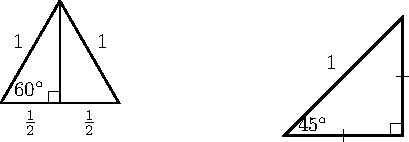
\includegraphics[width=0.5\columnwidth]{figures/0-5-fig_specialright.pdf}
    \end{center}
        \item Finally, we can organize all of the information about the special right
            triangles on a well-known organizational tool: the unit circle.  The $x$
            coordinate of each point is the cosine of the angle and the $y$ coordinate of
            each point is the sine of the angle.  
    \begin{center}
        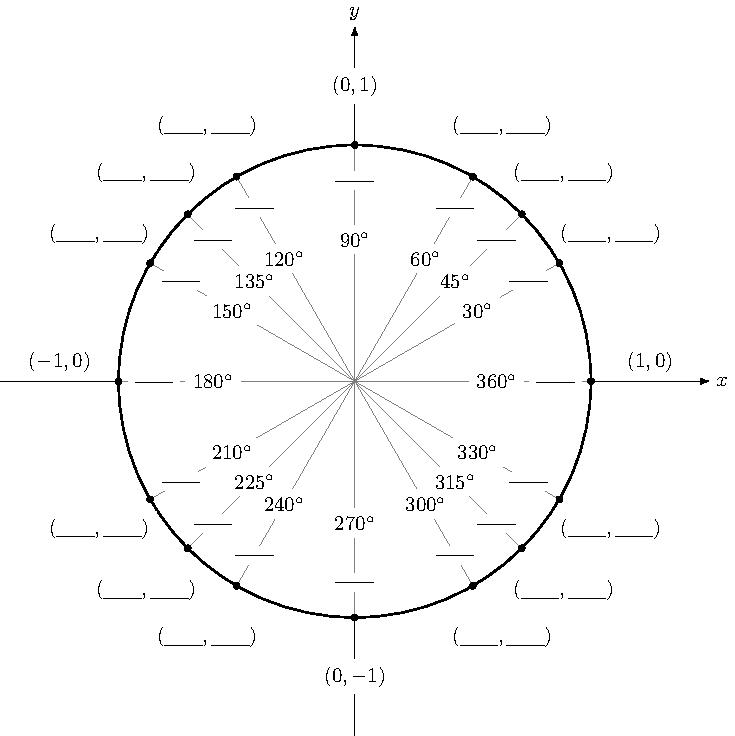
\includegraphics[width=0.7\columnwidth]{figures/0-5-UnitCircle.pdf}
    \end{center}
    \ea

\end{activity}
\begin{smallhint}
\end{smallhint}
\begin{bighint}
\end{bighint}
\begin{activitySolution}
    \begin{center}
        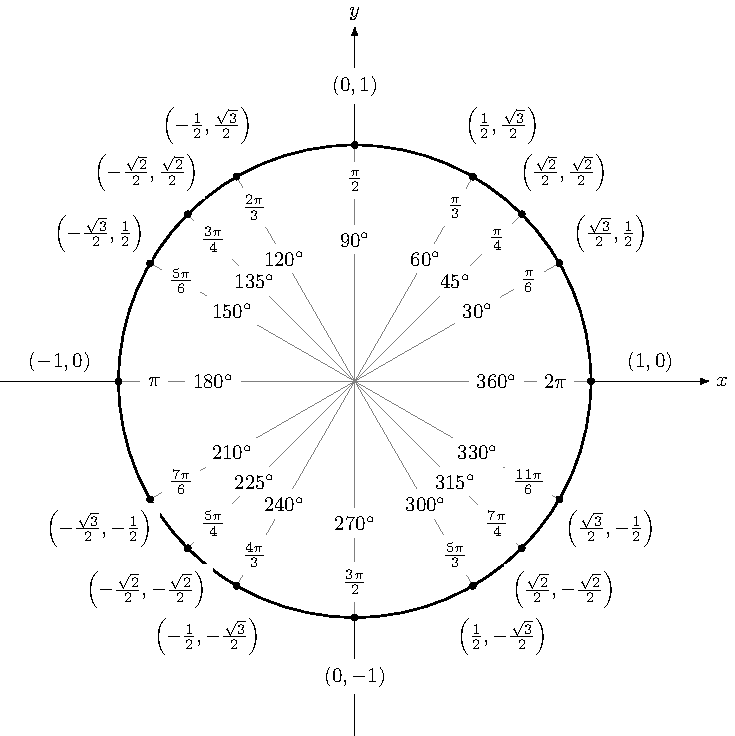
\includegraphics[width=0.6\columnwidth]{figures/0-5-UnitCircle_FilledIn.pdf}
    \end{center}
\end{activitySolution}

\aftera







\subsection*{Units}

Whenever we use mathematics in the real world, most numbers have units, like meters,
minutes, dollars, pounds, or degrees.  Units are a very useful tool that helps us
understand the meaning of the numbers that we are using.  For example, suppose we use the
following sinusoidal function to model the water level on a pier in the ocean as it
changes due to the tides during a certain day.
\[ w(t) = 4.3 \sin \left( 0.51 t + 0.82 \right) + 10.6 \]
This function isn't very useful to us unless we know what units the input $t$ must have
(Minutes?  Seconds?  Hours?  Days?) and what units the output $w$ will have (Centimeters?
Feet?  Meters?  Yards?).  In this case $t$ is in hours since midnight, and $w$ is in feet.
Now, we can evaluate the function at noon to find that the water level is $w(12) = 13.3$
feet.

\begin{callout}
    Here's how units work in equations:  
    \begin{itemize}
        \item If two numbers are equal, or if we add or subtract
            two numbers, they must have the same units:  3 seconds plus 5 feet doesn't make any sense.
        \item If we multiply or divide two numbers, both units go into the result:  6 meters divided by
            2 seconds equals a speed of 3 meters per second. 
    \end{itemize}
\end{callout}

The parameters in our water level function ($A = 4.3$, $B = 0.51$, $\phi = 0.82$, $C =
10.6$) all have units, which help us interpret their meaning.   The sine, cosine, and
tangent functions all take angles in radians as their input, and return numbers with no
units as output.  $C = 10.6$ must be in feet, because we add it to something else, and
then it equals the output, which is in feet.  Similarly $A = 4.3$ must also be in feet,
because the sine function does not have any units on its output.  $\phi = 0.82$ must be in
radians, because we add it to something else and use it as input to the sine function.
Similarly $0.51 t$ must be in radians.  However, we know that $t$ is in hours, so $B =
0.51$ must have units of radians per second.  





\begin{activity}\label{A:0.5.2}
Suppose the following sinusoidal function models the water level on a pier in the ocean as
it changes due to the tides during a certain day.
\[ w(t) = 4.3 \sin \left( 0.51 t + 0.82 \right) + 10.6 \]
\ba
\item Using the formula above, make a table showing the water level every two hours for a 24 hour period starting at midnight.
    \begin{center}
        \begin{tabular}[h!]{|c||c|c|c|c|c|c|c|c|c|c|c|c|c|}
            \hline
            time (hours) & 0 & 2 & 4 & 6 & 8 & 10 & 12 & 14 & 16 & 18 & 20 & 22 & 24 \\
            \hline
            water level (ft) & & & & & & & & & & & & & \\ \hline
        \end{tabular}
    \end{center}
\item Sketch a graph of this function using the data from your table in part (a).
    \begin{center}
        \begin{tikzpicture}
            \begin{axis}[ymin=0, ymax=20, xmin=0, xmax=24, domain=0:24,
                grid, xtick={2,4,6,8,10,12,14,16,18,20,22,24},
            ytick={0,2,4,6,8,10,12,14,16,18,20}, xlabel={time (hours)}, ylabel={water level
            (ft)}, xscale=1.25]
                \addplot[smooth] {0*x};
            \end{axis}
        \end{tikzpicture}
    \end{center}
\item What is the period of oscillation of this function? % Period $ = 2 \pi / B \approx  12.3$ hours.
\item What time is high tide?  % The sine function reaches a peak when its input is $\pi/2$.  So $0.51 t + 0.82 = \pi/2$ and $t = 1.47$ hours, or about 1:30 am.

\ea
\end{activity}\aftera







\subsection*{The Tangent Function}

The tangent function has a completely different shape than the sine and cosine functions because it is defined to be
\[ \tan \theta = \frac{\sin \theta}{\cos \theta} \]
as long as $\cos \theta \neq 0$, so that we don't have a divide-by-zero problem.  This
means that the tangent function is undefined at $\pm \pi/2, \pm 3 \pi/2, \cdots$, and the
function has vertical asymptotes at these points.
\begin{center}
    \begin{tikzpicture}
        \begin{axis}[axis lines=center, xlabel={$x$}, xmin=-7, xmax=7,
                ymin=-1.5, ymax=1.5, ytick={-1,1}, xtick={-6.28, -4.71, -3.14, -1.57,
                1.57, 3.14, 4.71, 6.28},
            xticklabels={$-2\pi$,$-\frac{3}{2}\pi$,$-\pi$,$-\frac{1}{2}\pi$,$\frac{1}{2}\pi$,$\pi$,$\frac{3}{2}\pi$,$2\pi$},
        grid, xscale=2, restrict y to domain=-3:3]
            \addplot[smooth, very thick, color=blue, domain=-6.5:6.5, samples=100] {tan(deg(x))};
            \draw (axis cs:1.7,1) node[anchor=south west]{$y = \tan(x)$};
            \draw[thick, dashed] (axis cs:-4.71,-1.5) -- (axis cs:-4.71,1.5);
            \draw[thick, dashed] (axis cs:4.71,-1.5) -- (axis cs:4.71,1.5);
            \draw[thick, dashed] (axis cs:-1.57,-1.5) -- (axis cs:-1.57,1.5);
            \draw[thick, dashed] (axis cs:1.57,-1.5) -- (axis cs:1.57,1.5);
        \end{axis}
    \end{tikzpicture}
\end{center}
% \resizebox{3in}{!}{\includegraphics{0-5-TrigonometricFunctions9.jpg}}
Because the tangent function blows up to infinity, we don't often fit tangent functions to real world data.

\subsection*{Inverse Sine Function}

Suppose we want to find the value of $x$ so that $\sin x = 0.75$.  To find this, we use an
inverse sine function, written as either $\arcsin$ or $\sin^{-1}$.  In this case
$\sin^{-1} 0.75 \approx 0.848$, because $\sin 0.848 \approx 0.75$.  The range of the sine
function only goes from $-1$ to $+1$, so that means the domain of $\arcsin$ only goes from
$-1$ to $+1$.  It is impossible to find a solution to $\sin x = 3$, because the sine
function doesn't go that high!

It is important to remember that the sine function repeats itself in the same pattern
again and again, every $2\pi$, so $x = 0.848$ is not the only solution to $\sin x = 0.75$.
Another solution is $x = 0.848 + 2 \pi \approx 7.13$.  Another solution is $x = 0.848 + 4
\pi \approx 13.4.$.  And of course we could subtract multiples of $2 \pi$ as well to get
$x = 0.848 - 2 \pi \approx -5.44$.  As a result, we have the $\arcsin$ function output the
value between $-\pi/2$ and $+\pi/2$.  This means that the arcsine function has a very
limited domain and range, only existing for $ -1 \leq x \leq 1$ and $-\pi/2 \leq y \leq
\pi/2$.
\begin{center}
    \begin{tikzpicture}
        \draw[thick, <->] (-2,0) -- (2,0) node[anchor=west]{$x$};
        \draw[thick, <->] (0,-2.25) -- (0,2.25) node[anchor=south]{$y=\sin^{-1}(x)$};
        \draw[color=blue, very thick, domain=-1.57:1.57] plot ({sin(deg(\x))},{\x});
        \draw (1,0) node[anchor=north]{$1$};
        \draw (-1,0) node[anchor=south]{$-1$};
        \draw (0,1.57) node[anchor=east]{$\pi/2$};
        \draw (0,-1.57) node[anchor=west]{$-\pi/2$};
        \draw[thick, dashed] (1,0) -- (1,1.57) -- (0,1.57);
        \draw[thick, dashed] (-1,0) -- (-1,-1.57) -- (0,-1.57);
        \draw (0,-2.25) node[anchor=north]{Domain: $-1\le x \le 1$, Range: $-\pi/2 \le y
        \le \pi/2$};
    \end{tikzpicture}
\end{center}

% \resizebox{2in}{!}{\includegraphics{0-5-TrigonometricFunctions10.jpg}}
Warning:  Even though we write the inverse sine function as $\sin^{-1} x$, it is a completely different thing than $1 / \sin x$.
\[ \sin^{-1}x \neq \frac{1}{\sin x} \]

\subsection*{Inverse Cosine Function}

We can define a similar inverse function for the cosine, which we call $\arccos$ or
$\cos^{-1}$.  The domain of this function is $-1 \leq x \leq 1$, and we choose the range
to be $0 \leq y \leq \pi$.
\begin{center}
    \begin{tikzpicture}
        \draw[thick, <->] (-2,0) -- (2,0) node[anchor=west]{$x$};
        \draw[thick, <->] (0,-1) -- (0,4) node[anchor=south]{$y=\cos^{-1}(x)$};
        \draw[color=blue, very thick, domain=0:3.14] plot ({cos(deg(\x))},{\x});
        \draw (1,0) node[anchor=north]{$1$};
        \draw (-1,0) node[anchor=north]{$-1$};
        \draw (0,3.14) node[anchor=west]{$\pi$};
        \draw[thick, dashed] (-1,0) -- (-1,3.14) -- (0,3.14);
        \draw (0,-1) node[anchor=north]{Domain: $-1\le x \le 1$, Range: $0 \le y
        \le \pi$};
    \end{tikzpicture}
\end{center}

% \resizebox{2in}{!}{\includegraphics{0-5-TrigonometricFunctions11.jpg}}

\subsection*{Inverse Tangent Function}

Recall that the tangent function has a range going all the way from negative infinity to
positive infinity, as $x$ goes from $-\pi/2$ to $+\pi/2$.  As a result, the inverse
tangent function has a domain of $-\infty < x < \infty$, and a range of $-\pi/2 \leq y
\leq \pi/2$.

\begin{center}
    \begin{tikzpicture}
        \draw[thick, <->] (-3,0) -- (3,0) node[anchor=west]{$x$};
        \draw[thick, <->] (0,-2.25) -- (0,2.25) node[anchor=south]{$y=\tan^{-1}(x)$};
        \draw[color=blue, very thick, domain=-1.25:1.25] plot ({tan(deg(\x))},{\x});
        \draw (0,1.57) node[anchor=south east]{$\pi/2$};
        \draw (0,-1.57) node[anchor=north west]{$-\pi/2$};
        \draw[thick, dashed] (-3,1.57) -- (3,1.57);
        \draw[thick, dashed] (-3,-1.57) -- (3,-1.57);
        \draw (0,-2.25) node[anchor=north]{Domain: $\mathbb{R}$, Range: $-\pi/2 < y
        < \pi/2$};
    \end{tikzpicture}
\end{center}
% \resizebox{2in}{!}{\includegraphics{0-5-TrigonometricFunctions12.jpg}}
% 
% 


\clearpage


\begin{summary}
\item Trigonometric functions are utilized to model periodic behavior such as tides,
    sound waves, or voltage through an electrical circuit.
\item Converting between radian measure and degree measure can be achieved by remembering
    that
    \[ 2\pi \text{ radians} = 360^\circ \]
\item for $f(t) = A \sin( B ( t - t_0) ) + C$ or $f(t) = A \sin( B t + \phi) + C$
\begin{itemize}
\item $A$ is the amplitude.  
\item $B$ is the angular frequency, which determines the period, with $B = \frac{2 \pi}{\mbox{Period}}$.  
\item $C$ is the average value.  
\item $t_0$ is the shift along the $t$ axis, a time when $f$ is at an average value and increasing
\item $\phi$ is the shift in radians, the angle at which the oscillations begin
\end{itemize}
\end{summary}


% exercises go here
\begin{exercises} 

\item What is the formula for a sinusoidal function that has a minimum at coordinates
    $(3,6)$ followed by a maximum at $(5,9)$?  %  1.5 \sin(\frac{ \pi}{2} (x-3)) + 7.5 
\begin{exerciseSolution}
\end{exerciseSolution}


\item For each of the following trigonometric functions find the amplitude, period, and
    phase shift.
    \begin{flalign*}
        a(x) &= -\sqrt{19} \sin\left(  7 \pi x + 18 \right) \\
        b(x) &= -15 \cos\left( 5\left( x+\frac{\pi}{2} \right) \right) \\
        c(x) &= -2 \cos\left( \frac{x}{7} \right) \\
        d(x) &= 5 \cos\left( 5x-\frac{\pi}{8} \right) \\
    \end{flalign*}

\item Write the equation of the trigonometric function shown in each plot below.
    \begin{center}
        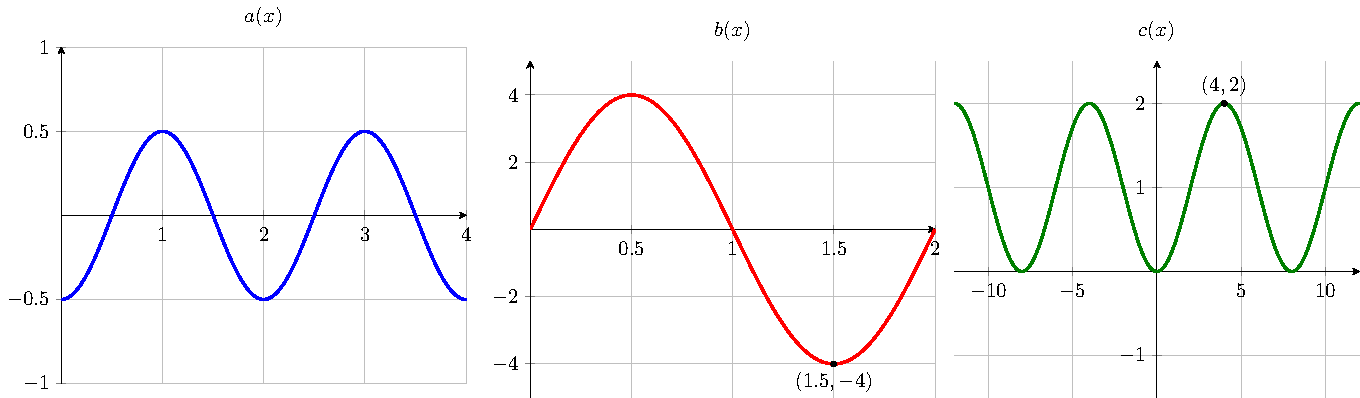
\includegraphics[width=0.99\columnwidth]{figures/0-5-fig13.pdf}
    \end{center}


\item If we take a sinusoidal function $f(t)= A \sin ( B (t - t_0)) + C$ and replace one of
    the parameters with a another function, say a linear function, we can create more
    complicated shapes.  Find formulas for the function plotted in the following graphs.

    \def\scl{0.9}
    \begin{center}
        \begin{tikzpicture}[scale=\scl]
            \begin{axis}[axis lines=center, xmin=0, xmax=20, ymin=0, ymax=15, domain=0:20,
                xlabel={$t$}, title={Plot A}, grid]
                \addplot[smooth, blue, very thick, samples=100] {2*cos(deg(x)) + 3 + 0.5*x};
            \end{axis}
        \end{tikzpicture}
        \begin{tikzpicture}[scale=\scl]
            \begin{axis}[axis lines=center, xmin=0, xmax=10, ymin=-25, ymax=25, domain=0:10,
                xlabel={$t$}, title={Plot B}, grid]
                \addplot[smooth, blue, very thick, samples=100] {3*x*sin(deg(3*x))};
            \end{axis}
        \end{tikzpicture}
        \begin{tikzpicture}[scale=\scl]
            \begin{axis}[axis lines=center, xmin=-10, xmax=10, ymin=-40, ymax=25, domain=-10:10,
                xlabel={$t$}, title={Plot C}, grid]
                \addplot[smooth, blue, very thick, samples=100] {15*cos(deg(2*x))+5-x^2};
            \end{axis}
        \end{tikzpicture}
        \begin{tikzpicture}[scale=\scl]
            \begin{axis}[axis lines=center, xmin=-10, xmax=10, ymin=-10, ymax=10, domain=-10:10,
                xlabel={$t$}, title={Plot D}, grid]
                \addplot[smooth, blue, very thick, samples=100]
                {5*cos(deg(x))+1*sin(deg(5*x))};
            \end{axis}
        \end{tikzpicture}
    \end{center}
\begin{exerciseSolution}
    \ba
        \item $f(t) = 2\cos(t) + 3 + 0.5*t$ over the range $[0,20]$
        \item $f(t) = 3t \sin(3t)$ over the range $[0,10]$
        \item $f(t) = 15\cos(2t) + 5-t^2$ over $[-10,10]$
        \item $f(t) = 5\cos(t) + \sin(5t)$
    \ea
\end{exerciseSolution}


\item The number of hours of daylight varies sinusoidally throughout the year.  The
    maximum occurs on the summer solstice, June 21, when we have 15 hours and 50 minutes
    of daylight.  The minimum occurs on the winter solstice, December 21, when we have
    only 8 hours and 33 minutes of daylight.  Find the formula for a function to describe
    this.  The input to your function should be $d$, the number of days since the
    beginning of the year, so that $d = 5$ on January 5.  The output of your function
    should be the amount of daylight, in minutes.  Assume that this is not a leap year.
    Hint:  Because we know the date of maximum, it is easier to write this in terms of a
    cosine function.
    % f(d) = 218.5 cos( \frac{2 \pi}{365} (d – 172) ) + 731.5

\begin{exerciseSolution}
\end{exerciseSolution}



\end{exercises}
\afterexercises





\clearpage

% \section{Powers, Polynomials, and Rational Functions} \label{S.0.6.PowersPolysRationals}


\vspace*{-14 pt}
\framebox{\hspace*{3 pt}
\parbox{6.25 in}
{\begin{goals}
	\item What are power, polynomial, and rational functions?
	\item How can be build polynomial functions from data?
	\item What microscopic/macroscopic behavior can we expect from polynomial and rational functions?
 \end{goals}} 
\hspace*{3 pt}}


% \begin{web}
% \item \href{https://www.khanacademy.org/math/algebra2/polynomial_and_rational}{Khan
%     Playlist: Polynomial and rational functions}
% \item
%     \href{https://www.khanacademy.org/math/algebra2/polynomial_and_rational/rational_funcs_tutorial/v/adding-and-subtracting-rational-expressions}{Khan
%     Playlist: Rational functions}
% \end{web}

\nin \hrulefill


\subsection*{Introduction}

Polynomial functions play an important role in mathematics.  They are generally simple to compute (requiring only computations that can be done by hand) and can be used to model many real-world phenomena.  In fact, scientists and mathematicians frequently simplify complex mathematical models by substituting a polynomial model that is "close enough" for their purposes.

In this section, we will study the graphs of select polynomial and rational functions to identify their important features.  The goal of this section is to build a mathematical intuition about how a small class of 'convenient' functions behave so that later we can see how calculus can be used to determine the behavior of arbitrary functions.

\begin{pa} \label{PA:0.6}
    
Figure \ref{fig:0.6.PA} shows the graphs of two different functions.  Suppose that you were to graph a line anywhere along each of the two graphs.

\begin{enumerate}
	\item Is it possible to draw a line that does not intersect the graph of $f$? $g$?
	\item Is it possible to draw a line that intersects the graph of $f$ an even number of times?
	\item Is it possible to draw a line that intersects the graph of $g$ an odd number of times?
	\item What is the fewest number of intersections that your line could have with the graph of $f$? with $g$?
	\item What is the largest number of intersections that your line could have with the graph of $f$? with $g$?
	\item How many times does the graph of $f$ change directions? How many times does the graph of $g$ change directions?
\end{enumerate}

\begin{figure}[ht!]

	\begin{center}
		\begin{tikzpicture}[scale=0.75]
			[line cap=round,line join=round,>=triangle 45,x=1.0cm,y=1.0cm] 
			\draw[<->,color=black] (-4.418087504107611,0.0) -- (5.504275777242757,0.0); \foreach \x in {-4.0,-3.0,-2.0,-1.0,1.0,2.0,3.0,4.0,5.0} 
			\draw[shift={(\x,0)},color=black] (0pt,2pt) -- (0pt,-2pt); 
			\draw[<->] (0.0,-2.486833997057605) -- (0.0,5.09438316608086); \foreach \y in {-2.0,-1.0,1.0,2.0,3.0,4.0,5.0} 
			\draw[shift={(0,\y)},color=black] (2pt,0pt) -- (-2pt,0pt); 
			\clip(-4.418087504107611,-2.486833997057605) rectangle (5.504275777242757,5.09438316608086); 
			\draw[color=blue, very thick,smooth,samples=100,domain=-3.3:4.5]
			plot(\x,{((\x)-1.1)^(2.0)*((\x)-3.6)*((\x)+1.5)*((\x)-4.2)*((\x)+2.2)*((\x)+3.1)/100.0});
			\begin{scriptsize}
				\draw[color=black] (5,4.671245463952202) node {$f(x)$};
			\end{scriptsize}
		\end{tikzpicture}
		\begin{tikzpicture}[scale=0.75]
			[line cap=round,line join=round,>=triangle 45,x=1.0cm,y=1.0cm] 
			\draw[<->,color=black] (-4.418087504107611,0.0) -- (5.504275777242757,0.0); \foreach \x in {-4.0,-3.0,-2.0,-1.0,1.0,2.0,3.0,4.0,5.0} 
			\draw[shift={(\x,0)},color=black] (0pt,2pt) -- (0pt,-2pt); 
			\draw[<->,color=black] (0.0,-2.486833997057605) -- (0.0,5.09438316608086); \foreach \y in {-2.0,-1.0,1.0,2.0,3.0,4.0,5.0} 
			\draw[shift={(0,\y)},color=black] (2pt,0pt) -- (-2pt,0pt); 
			\clip(-4.418087504107611,-2.486833997057605) rectangle (5.504275777242757,5.09438316608086); 
			\draw[color=blue, very thick,smooth,samples=100,domain=-4:5]
			plot(\x,{((\x)-1.1)*((\x)-3.6)*((\x)+1.5)*((\x)-4.2)*((\x)+2.2)*((\x)+3.1)/100.0});
			\begin{scriptsize}
				\draw[color=black] (5.1,4.671245463952202) node {$g(x)$};
			\end{scriptsize}
		\end{tikzpicture} 
	\end{center}      
\caption{$f(x)$ and $g(x)$ for the preview activity.}
\label{fig:0.6.PA}
\end{figure}


\end{pa} \afterpa


\subsection*{Power Functions}

Power functions are fundamental building blocks for many very useful functions.  In their simplest form, power functions describe situations when the dependent variable is directly proportional to a power of the independent variable.

\begin{definition}
% Power Functions
A {\bf power function} has the form
	\[ 
		f(x) = kx^{n}, \qquad \mbox{where } k \mbox{ and } n \mbox{ are constant.}
	\]
\end{definition}


\begin{figure}[ht!]
	\begin{center}
% 		\begin{tikzpicture}%[scale=0.75]
% 			\begin{axis}[axis lines=center, xlabel={$x$}, ylabel={$y$},
% 				domain=-2.5:2.5,ymin=-15,ymax=15,xmin=-2.75,xmax=2.75]
% 				\addplot[smooth, very thick, blue, samples=150] {x}
% 					node[above]{$x$};
% 				\addplot[smooth, very thick, red, samples=150] {x^3}
% 					[below right] node[pos=0.9]{$x^3$};
% 				\addplot[smooth, very thick, black, samples=150] {x^5}
% 					[left] node[pos=0.57]{$x^5$};
% 			\end{axis}
% 		\end{tikzpicture}
% 		\begin{tikzpicture}%[scale=0.75]
% 			\begin{axis}[axis lines=center, xlabel={$x$}, ylabel={$y$},
% 				domain=-2.5:2.5,ymin=-10,ymax=15,xmin=-2.75,xmax=2.75]
% 				\addplot[smooth, very thick, blue, samples=150] {x^2}
% 					node[above]{$x^2$};
% 				\addplot[smooth, very thick, red, samples=150] {x^4} 
% 					[below right] node[pos=0.67]{$x^4$}; 				
% 				\addplot[smooth, very thick, black, samples=150] {x^6}
%  					[above left] node[pos=0.525]{$x^6$};
% 			\end{axis}
% 		\end{tikzpicture}     
        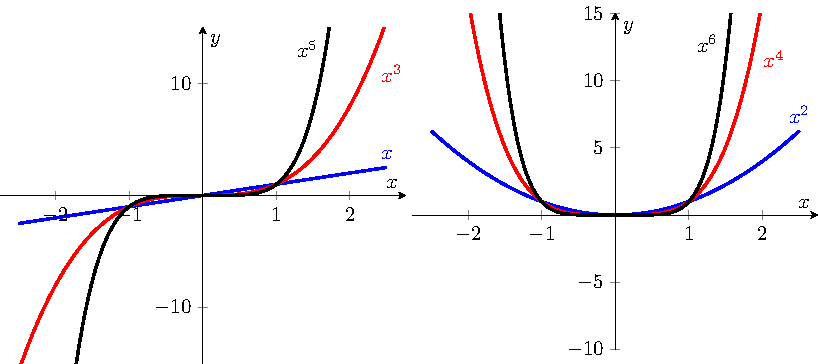
\includegraphics[width=0.9\columnwidth]{figures/0-6-fig2.pdf}
	\end{center}     
\caption{Positive odd powers of $x$ (left) and positive even powers of $x$ (right)}     
\label{F:0.6.Ex1} 
\end{figure}

For odd values of $n$, the graphs of $x^{n}$ are always increasing.  For even values of
$n$, the graphs of $x^{n}$ decrease until $x=0$ and then increase afterwards. See Figure
\ref{F:0.6.Ex1} for several examples of power functions. We can classify the {\it end
behavior} of the graphs by describing what happens as $x\to\infty$ and as $x\to-\infty$.
For odd $n$, $x^{n}\to -\infty$ as $x\to-\infty$ and $x^{n}\to\infty$ as $x\to\infty$.
Graphs of odd power functions go in opposite directions on the left and right.  For even
$n$, $x^{n}\to \infty$ as $x\to-\infty$ and $x^{n}\to\infty$ as $x\to\infty$.  Graphs of
even power functions go in the same direction on the left and right.

\begin{activity}\label{A:0.6.1}
Power functions and exponential functions appear somewhat similar in their formulas, but behave differently in many ways.  

\ba
% \begin{itemize}
	\item Compare the functions $f(x)=x^2$ and $g(x)=2^x$ by graphing both functions in several viewing windows.  Find the points of intersection of the graphs.  Which function grows more rapidly when $x$ is large?
    \item Compare the functions $f(x)=x^{10}$ and $g(x)=2^x$ by graphing both functions in several viewing windows.  Find the points of intersection of the graphs.  Which function grows more rapidly when $x$ is large?
	\item Make a conjecture: As $x\to\infty$, which dominates, $x^n$ or $a^x$?
	\item Suppose you are offered a job that lasts one month.  You have the option of being paid in one of two ways: (1) One million dollars at the end of the month; or (2) One cent on the first day of the month, two cents on the second day, four cents on the third day, and, in general, $2^{n-1}$ cents on the $n^{th}$ day.  Which option should you choose?
	\item How much different (shorter or longer) would the work period need to be for your answer to the previous question change?
% \end{itemize}
        \ea

\end{activity}\aftera


\subsection*{Polynomial Functions} 

\begin{definition}
% Polynomial Functions
A {\bf polynomial function} is a function of the form
	\[
		p(x)=a_{n}x^{n} + a_{n-1}x^{n-1}+\cdots + a_{1}x + a_{0}
	\]
where $n$ is a nonnegative integer and $a_{n}\ne 0$.  Here $n$ is the {\it degree} of the
polynomial, and $a_{n}$, $a_{n-1}$, \ldots, $a_{1}$, $a_{0}$ are the {\it coefficients}.
\end{definition}

When we study the graphs of functions, there are several common features we're interested in.  
\begin{itemize}
	\item How does the graph behave as $x\to\infty$ and as $x\to-\infty$? (Does it grow without bound? Does it level off? Does it oscillate?) 
	\item Where does the graph cross the $x$-axis? How many times? 
	\item Where does the graph change directions? How many times?
\end{itemize}

For many functions, these questions can be difficult to answer and require specialized
mathematics (like Calculus for example).  For polynomials, though, there are some
relatively simple results.  First, the end behavior of a polynomial is determined by its
degree and the sign of the lead coefficient.  Polynomials with even degree behave like
power functions with even degree, and polynomials with odd degree behave like power
functions like odd degree. Figures \ref{F:0.6.PolyEndBehavior} and
\ref{F:0.6.PolyEndBehavior2} demonstrate this for two different fourth degree polynomials.

% \def\scl{0.75}
\begin{figure}[ht!]
	\begin{center}
% 		\begin{tikzpicture}[line cap=round,line join=round,>=triangle 45, x=0.5cm,
%             y=0.006cm, scale=\scl] 
% 			\draw[<->,color=black] (-6,0.0) -- (7,0.0); 
% 			\foreach \x in {-4,-2,2,4,6} 
% 			\draw[shift={(\x,0)},color=black] (0pt,2pt) -- (0pt,-2pt) node[below] {\footnotesize $\x$}; 
% 			\draw[<->,color=black] (0.0,-100) -- (0.0,850); 
% 			\foreach \y in {,800} 
% 			\draw[shift={(0,\y)},color=black] (2pt,0pt) -- (-2pt,0pt) node[left] {\footnotesize $\y$}; 
% 			\draw[color=black] (0pt,-10pt) node[right] {\footnotesize $0$}; 
% 			\clip(-6,-200) rectangle (7,850); 
%             \draw[very thick, blue, smooth,samples=100,domain=-6:7] plot(\x,{(\x)^(4.0)}); 
% 			\begin{scriptsize} 
% 				\draw[color=black] (-0.5,-150) node {$y=x^{4}$}; 
% 			\end{scriptsize} 
% 		\end{tikzpicture}   
% 		\begin{tikzpicture}[line cap=round,line join=round,>=triangle 45, x=0.5cm, y=0.006cm, scale=\scl] 
% 			\draw[<->,color=black] (-6,0.0) -- (7,0.0); 
% 			\foreach \x in {-4,-2,2,4,6} 
% 			\draw[shift={(\x,0)},color=black] (0pt,2pt) -- (0pt,-2pt) node[below] {\footnotesize $\x$}; 
% 			\draw[<->,color=black] (0.0,-100) -- (0.0,850); 
% 			\foreach \y in {,800} 
% 			\draw[shift={(0,\y)},color=black] (2pt,0pt) -- (-2pt,0pt) node[left] {\footnotesize $\y$}; 
% 			\draw[color=black] (0pt,-10pt) node[right] {\footnotesize $0$}; 
% 			\clip(-6,-200) rectangle (7,850); 
% 			\draw[very thick, blue, smooth,samples=100,domain=-6:7] plot(\x,{(\x)^(4.0)-2.0*(\x)^(3.0)-12.0*(\x)^(2.0)+3.0*(\x)-4.0}); 
% 			\begin{scriptsize} 
% 				\draw[color=black] (-0.5,-150) node {$y=x^{4} - 2x^{3} - 12x^{2} + 3x - 4$}; 
% 			\end{scriptsize} 
% 		\end{tikzpicture}
        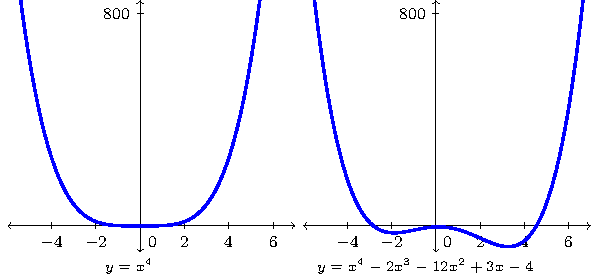
\includegraphics[width=0.8\columnwidth]{figures/0-6-fig3.pdf}
	\end{center}      
\caption{Local behavior of two fourth-degree polynomials.  At this level, we can clearly see the differences between these two functions.}
\label{F:0.6.PolyEndBehavior}
\end{figure}

\begin{figure}[ht!]
	\begin{center}
% 		\begin{tikzpicture}[line cap=round,line join=round,>=triangle 45, x=1.5cm, y=0.35cm, scale=\scl] 
% 			\draw[<->,color=black] (-2,0.0) -- (2,0.0); 
% 			\foreach \x in {-20,-10,10,20} 
% 			\draw[shift={(\x/10,0)},color=black] (0pt,2pt) -- (0pt,-2pt) node[below] {\footnotesize $\x$}; 
% 			\draw[->,color=black] (0.0,-2) -- (0.0,15); 
% 			\draw[shift={(0,14)},color=black] (2pt,0pt) -- (-2pt,0pt) node[left] {\footnotesize $160,000$}; 
% 			\draw[color=black] (0pt,-10pt) node[right] {\footnotesize $0$}; 
% 			\clip(-2,-4) rectangle (2,15); 
% 			\draw[very thick, blue, smooth,samples=100,domain=-2:2] plot(\x,{(\x)^(4.0)}); 
% 			\begin{scriptsize} 
% 				\draw[color=black] (-0.5,-3) node {$y=x^{4}$}; 
% 			\end{scriptsize} 
% 		\end{tikzpicture}  
% 		\begin{tikzpicture}[line cap=round,line join=round,>=triangle 45, x=1.5cm, y=0.35cm, scale=\scl] 
% 			\draw[<->,color=black] (-2,0.0) -- (2,0.0); 
% 			\foreach \x in {-20,-10,10,20} 
% 			\draw[shift={(\x/10,0)},color=black] (0pt,2pt) -- (0pt,-2pt) node[below] {\footnotesize $\x$}; 
% 			\draw[->,color=black] (0.0,-2) -- (0.0,15); 
% 			\draw[shift={(0,14)},color=black] (2pt,0pt) -- (-2pt,0pt) node[left] {\footnotesize $160,000$}; 
% 			\draw[color=black] (0pt,-10pt) node[right] {\footnotesize $0$}; 
% 			\clip(-2,-4) rectangle (2,15); 
% 			\draw[very thick, blue, smooth,samples=100,domain=-2:2] plot(\x,{(\x)^(4.0)}); 
% 			\begin{scriptsize} 
% 				\draw[color=black] (-0.5,-3) node {$y=x^{4} - 2x^{3} - 12x^{2} + 3x - 4$}; 
% 			\end{scriptsize} 
% 		\end{tikzpicture}  
        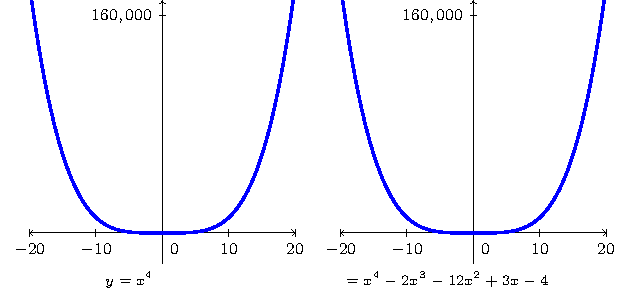
\includegraphics[width=0.8\columnwidth]{figures/0-6-fig4.pdf}
	\end{center}      
\caption{Long-term behavior of two fourth-degree polynomials.  At this scale, the two functions are nearly indistinguishable.}
\label{F:0.6.PolyEndBehavior2}
\end{figure}

\begin{theorem}
%Roots of polynomials
	A polynomial of degree $n$ has at most $n$ real zeros and at most $n-1$ turning points.\label{T:0.6.1}
\end{theorem}

\begin{theorem}\label{T:0.6.2}
%Polynomial roots and factors
	Let $p(x)$ be a polynomial.  If $x = a$ is a zero of $p$ (i.e. $p(a)=0$), then $(x-a)$ is a factor of $p$.
\end{theorem}

Theorems \ref{T:0.6.1} and \ref{T:0.6.2} are each fairly simple to state but very powerful.  Theorem \ref{T:0.6.1} gives us a quick way to determine the degree of a polynomial from its graph and is frequently used to determine how many solutions to expect from certain types of equations.  
Theorem \ref{T:0.6.2} provides us with a way to construct polynomials that pass through specific points.  

\begin{activity}\label{A:0.6.2}
	For each of the following graphs, find a possible formula for the polynomial of lowest degree that fits the graph.
    \def\scl{0.7}
				\begin{center}
%                     \begin{tikzpicture}[scale=\scl]
%                         \begin{axis}[axis lines=center, xmin=-4, xmax=2, ymin=-5, ymax=2,
%                             title={Plot (a)}]
%                             \addplot[very thick, blue, smooth,samples=100,domain=-4.0:2.0] {((x)-1.0)*((x)+3.0)};
%                         \end{axis}
%                     \end{tikzpicture}
%                     \begin{tikzpicture}[scale=\scl]
%                         \begin{axis}[axis lines=center, xmin=-3, xmax=3.5, ymin=-8.5, ymax=6,
%                             title={Plot (b)}, ytick={-8,-6,-4,-2,2,4,6}]
%                             \addplot[very thick, blue, smooth,samples=100,domain=-3:3.5] {0-((x)+2.0)*((x)-3.0)*((x)-1.0)};
%                         \end{axis}
%                     \end{tikzpicture}
%                     \begin{tikzpicture}[scale=\scl]
%                         \begin{axis}[axis lines=center, xmin=-2, xmax=3, ymin=-3, ymax=2,
%                             title={Plot (c)}]
%                             \addplot[very thick, blue, smooth,samples=100,domain=-2:3] {((x)+1.0)*((x)-2.0)*((x)-1.0)*((x)-1.0)};
%                         \end{axis}
%                     \end{tikzpicture}
% % 					\begin{tikzpicture}[line cap=round,line join=round,>=triangle 45, x=1.0cm, y=0.86cm] 
% % 						\draw[->,color=black] (-4.0,0.0) -- (2.0,0.0);
% % 						\foreach \x in {-4,-3,-2,-1,1}
% % 						\draw[shift={(\x,0)},color=black] (0pt,2pt) -- (0pt,-2pt) node[below] {\footnotesize $\x$};
% % 						\draw[->,color=black] (0.0,-5.0) -- (0.0,2.0);
% % 						\foreach \y in {-5,-4,-3,-2,-1,1}
% % 						\draw[shift={(0,\y)},color=black] (2pt,0pt) -- (-2pt,0pt) node[left] {\footnotesize $\y$};
% % 						\draw[color=black] (0pt,-10pt) node[right] {\footnotesize $0$};
% % 						\clip(-4.0,-5.0) rectangle (2.0,2.0);
% % 						\draw[very thick, blue, smooth,samples=100,domain=-4.0:2.0] plot(\x,{((\x)-1.0)*((\x)+3.0)});
% % 					\end{tikzpicture}   
% % 					\begin{tikzpicture}[line cap=round,line join=round,>=triangle 45, x=0.86cm, y=0.33cm] 
% % 						\draw[<->,color=black] (-3.5,0.0) -- (3.5,0.0); 
% % 						\foreach \x in {-3,-2,-1,1,2,3} 
% % 						\draw[shift={(\x,0)},color=black] (0pt,2pt) -- (0pt,-2pt) node[below] {\footnotesize $\x$}; 
% % 						\draw[->,color=black] (0.0,-10) -- (0.0,8); 
% % 						\foreach \y in {-8,-6,-4,-2,2,4,6}
% % 						\draw[shift={(0,\y)},color=black] (2pt,0pt) -- (-2pt,0pt) node[left] {\footnotesize $\y$}; 
% % 						\draw[color=black] (0pt,-10pt) node[right] {\footnotesize $0$}; 
% % 						\clip(-3.5,-10) rectangle (3.5,8); 
% % 						\draw[very thick, blue, smooth,samples=100,domain=-3.5:3.5] plot(\x,{0-((\x)+2.0)*((\x)-3.0)*((\x)-1.0)});
% % 					\end{tikzpicture}   
% % 					\begin{tikzpicture}[line cap=round,line join=round,>=triangle 45, x=1.2cm, y=1.1cm] 
% % 						\draw[<->,color=black] (-2,0.0) -- (3,0.0); 
% % 						\foreach \x in {-2,-1,1,2,3} 
% % 						\draw[shift={(\x,0)},color=black] (0pt,2pt) -- (0pt,-2pt) node[below] {\footnotesize $\x$}; 
% % 						\draw[->,color=black] (0.0,-3.5) -- (0.0,2); 
% % 						\foreach \y in {-3,-2,-1,1,2}
% % 						\draw[shift={(0,\y)},color=black] (2pt,0pt) -- (-2pt,0pt) node[left] {\footnotesize $\y$}; 
% % 						\draw[color=black] (0pt,-10pt) node[right] {\footnotesize $0$}; 
% % 						\clip(-2,-3.5) rectangle (3,2); 
% % 						\draw[very thick, blue, smooth,samples=100,domain=-2:3] plot(\x,{((\x)+1.0)*((\x)-2.0)*((\x)-1.0)*((\x)-1.0)}); 
% % 					\end{tikzpicture}   
                    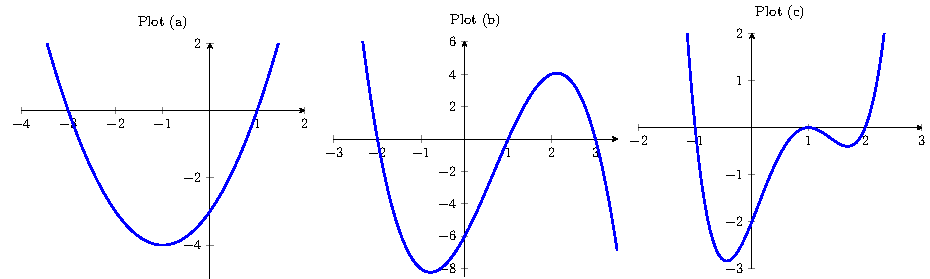
\includegraphics[width=0.99\columnwidth]{figures/0-6-fig5.pdf}
				\end{center}      
\end{activity}
\begin{smallhint}
How many roots are there and how do the ends behave?
\end{smallhint}
\begin{bighint}
    You may want to use Theorems \ref{T:0.6.1} and \ref{T:0.6.2} to determine the degree
    of the polynomial as well as the roots and factors.
\end{bighint}
\begin{activitySolution}
   \ba
        \item This function clearly has two roots and the ends show the same behavior.
            This indicates that this is likely a degree 2 polynomial (a quadratic).  Based
            on the roots $x=-2$ and $x=1$ the factors are $(x+2)$ and $(x-1)$ so the
            polynomial is of the form $a(x) = C(x+2)(x-1)$.  Finally, it appears that the
            point $(-1,-4)$ is on the curve so $C=2$ and the polynomial is 
            \[ a(x) = 2(x+2)(x-1). \]
        \item This function clearly has three roots and the ends show the opposite
            behavior.  Since the right-hand side of the function tends down we expect a
            negative leading coefficient.  Based on the roots $x=-2$, $x=1$, and $x=3$ the
            factors are $(x+2)$, $(x-1)$, and $(x-3)$ and the polynomial takes the form
            $b(x) = C(x+2)(x-1)(x-3)$.  The point $(-1,-8)$ appears to be on the graph so
            $C = -1$ and the polynomial is
            \[ b(x) = -(x+2)(x-1)(x-3). \]
        \item This function clearly has three roots but the end behavior indicates an even
            degree polynomial.  The root at $x=1$ is special since we do not cross the $x$
            axis.  Hence, the factors are $(x+1)$, $(x-1)$, $(x-1)$, and $(x-2)$.  Notice
            that the $(x-1)$ root is listed twice, and hence the polynomial takes the form
            $c(x) = C(x+1)(x-1)^2(x-2)$.  The point $(0,-2)$ appears to be on the graph so
            $C = 1$ and the polynomial is
            \[ c(x) = (x+1)(x-1)^2(x-2). \]
   \ea
\end{activitySolution}

\aftera


\subsection*{Rational Functions}

\begin{definition}
	% Rational Functions
	A {\bf rational function} is a ratio of two polynomial functions
		\[ 
			f(x) = P(x)/Q(x)
		\]
	where $P$ and $Q$ are polynomials.  The domain is the set of all real numbers for which $Q(x)\ne 0$
\end{definition}

\begin{definition}
	%Horizontal and Vertical Asymptotes
	A function $f$ has a {\bf horizontal asymptote} $y = a$ if the distance between the $f$ and the line $y=a$ becomes arbitrarily small when $x$ becomes sufficiently large.
	Alternatively, a horizontal asymptote is a line that a function approaches as $x \to \infty$ or as $x \to -\infty$. 
\end{definition}

\begin{definition}
    A function $f$ has a {\bf vertical asymptote} at a point $x = b$ if the function becomes arbitrarily large as $x \to b$.
\end{definition}

The graphs of rational functions may have vertical asymptotes only where the denominator is zero.  However, there are many examples of rational functions that do not have a vertical asymptote even at a point where the denominator is zero. (For instance, try graphing the function $f(x)=\displaystyle{\frac{x^{2}-1}{x-1}}$).

\begin{activity}\label{A:0.6.3}
% The purpose of this activity is to prompt students to start thinking about vertical asymptotes (and division by 0) in terms of limits.  
\ba
		\item Suppose $f(x) = x^{2}+ 3x + 2$ and $g(x) = x - 3$.  
			\begin{enumerate}
                \item[(i)] What is the behavior of the function $h(x) = \displaystyle{\frac {f(x)}{g(x)}}$ near $x = -1$? (i.e. what happens to $h(x)$ as $x\to -1$?) near $x = -2$? near $x = 3$?
                \item[(ii)] What is the behavior of the function $k(x) = \displaystyle{\frac {g(x)}{f(x)}}$ near $x = -1$? near $x = -2$? near $x = 3$?
			\end{enumerate}
		\item Suppose $f(x) = x^{2} - 9$ and $g(x) = x - 3$.  
			\begin{enumerate}
                \item[(i)] What is the behavior of the function $h(x) = \displaystyle{\frac {f(x)}{g(x)}}$ near $x = -3$? (i.e. what happens to $h(x)$ as $x\to -3$?) near $x = 3$?
                \item[(ii)] What is the behavior of the function $k(x) = \displaystyle{\frac {g(x)}{f(x)}}$ near $x = -3$? near $x = 3$?
			\end{enumerate}
% 		\item Suppose $f(x) = \sin{x}$ and $g(x) = x$.
% 			\begin{enumerate}
%                 \item[(i)] What is $f(0)$? What is $g(0)$?
%                 \item[(ii)] What is the behavior of the function $h(x) = \displaystyle{\frac {f(x)}{g(x)}}$ near $x = 0$? (i.e. what happens to $h(x)$ as $x\to 0$?)
%                 \item[(iii)] What is the behavior of the function $k(x) = \displaystyle{\frac {g(x)}{f(x)}}$ near $x = 0$?
% 			\end{enumerate}
\ea

\end{activity}
\begin{smallhint}
    Watch carefully for division by zero.  That is where a vertical asymptote is possible.
\end{smallhint}
\begin{bighint}
    Watch carefully for division by zero.  That is where a vertical asymptote is possible.
\end{bighint}
\begin{activitySolution}
   \ba
        \item For $f(x) = x^2+3x+2$ and $g(x) = x-3$ when we form the function $h(x) =
            f(x)/g(x)$ we get $h(x) = \frac{x^2+3x+2}{x-3}$.  Notice that $h(-1) = 0$ and
            $h(-2) = 0$ since $f(-1) = f(-2) = 0$ and $g(-2) \neq 0$.  At $x=3$, on the
            other hand, $g(x) = 0$ and there is a vertical asymptote on the function
            $h(x)$.

            For $k(x) = g(x) / f(x)$.  The vertical asymptotes occur at $x=-2$ and $x=-1$
            and a zero occurs at $x=3$.
        \item For $f(x) = x^2-9$ and $g(x) = x-3$ we see immediately that $f(x)$ can be
            factored to $f(x) = (x-3)(x+3)$ and hence the function $h(x) = f(x)/g(x)$
            simplifies to $h(x) = x+3$ when $x$ is not $3$.  When $x=3$ there is a
            discontinuity in the graph but this is not a vertical asymptote since the
            discontinuity can be removed algebraically.

            For $k(x) = g(x)/f(x)$ we simplify to $k(x) = 1/(x+3)$ when $x$ is not $3$.
            Therefore there is a vertical asymptote at $x=-3$ and a removable
            discontinuity at $x=3$.
   \ea
\end{activitySolution}

\aftera
  % Vertical Asymptotes and 0/0

\begin{activity}\label{A:0.6.4}

%The purpose of this activity is to encourage students to think of horizontal asymptotes in terms of "dominance" of the numerator over denominator (or vice versa).  
	
\ba
		\item Suppose $f(x) = x^{3} + 2x^{2}-x + 7$ and $g(x) = x^{2} + 4x + 2$.  
			\begin{enumerate}
				\item Which function dominates as $x \to \infty$?
				\item What is the behavior of the function $h(x) = \displaystyle{\frac {f(x)}{g(x)}}$ as $x \to \infty$?
				\item What is the behavior of the function $h(x) = \displaystyle{\frac {g(x)}{f(x)}}$ as $x \to \infty$?
			\end{enumerate}
		\item Suppose $f(x) = 2x^{4} - 5x^{3} + 8x^{2} - 3x - 1$ and $g(x) = 3x^{4} - 2x^{2} + 1$
			\begin{enumerate}
				\item Which function dominates as $x \to \infty$?
				\item What is the behavior of the function $h(x) = \displaystyle{\frac {f(x)}{g(x)}}$ as $x \to \infty$?
				\item What is the behavior of the function $h(x) = \displaystyle{\frac {g(x)}{f(x)}}$ as $x \to \infty$?
			\end{enumerate}
        \item Suppose $f(x) = e^{x}$ and $g(x) = x^{10}$.
			\begin{enumerate}
				\item Which function dominates as $x \to \infty$ as $x \to \infty$?
				\item What is the behavior of the function $h(x) = \displaystyle{\frac {f(x)}{g(x)}}$ as $x \to \infty$?
				\item What is the behavior of the function $h(x) = \displaystyle{\frac {g(x)}{f(x)}}$ as $x \to \infty$?
			\end{enumerate}
\ea

\end{activity}\aftera
  % Horizontal Asymptotes and infinity/infinity.

\begin{activity}\label{A:0.6.5}
	For each of the following functions, determine (1) whether the function has a horizontal asymptote, and (2) whether the function crosses its horizontal asymptote.
\ba
		\item $f(x)=\displaystyle{\frac {x+3}{5x-2}}$
		\item $g(x)=\displaystyle{\frac {x^{2}+2x-1}{x-1}}$
		\item $h(x)=\displaystyle{\frac {x+1}{x^{2}+2x-1}}$
\ea
\end{activity}
\begin{smallhint}
    A horizontal asymptote occurs where the function approaches a value  as $x\to\infty$.
    It is possible for a function to cross a horizontal asymptote.
\end{smallhint}
\begin{bighint}
    A horizontal asymptote occurs where the function approaches a value  as $x\to\infty$.
    It is possible for a function to cross a horizontal asymptote.
\end{bighint}
\begin{activitySolution}
   \ba
        \item For $f(x) = \frac{x+3}{5x-2}$ the degrees of the two polynomials are both $1$
            so the numerator and denominator grow at the same rate.  The horizontal
            asymptote will be the ratio of the coefficients: $f(x) \to
            \frac{1}{5}$ as $x \to \infty$.  The graph does not cross the horizontal
            asymptote.
        \item In this case where $g(x) = \frac{x^2+2x-1}{x-1}$ the degree of the numerator
            is larger than the degree of the denominator so $g(x) \to \infty$ as
            $x\to\infty$ and there is no horizontal asymptote.
        \item In this case where $h(x) = \frac{x+1}{x^2+2x-1}$ the degree of the
            denominator is larger than the degree of the numerator so $h(x) \to 0$ as $x
            \to \infty$.  Therefore, there is a horizontal asymptote at $y=0$.  Observe
            that $h(-1) = 0$ so the function's graph does indeed cross the horizontal
            asymptote.
   \ea
\end{activitySolution}

\aftera
  % Crossing Horizontal Asymptotes



\begin{summary}
	\item A polynomial of degree $n$ has at most $n$ real zeros and $n-1$ turning points.
	\item The degree of a polynomial function determines the end behavior of its graph.  If the degree of a polynomial is even, then the end behavior is the same in both directions.  If the degree of a polynomial is odd, then the end behavior on the left is the opposite of the behavior on the right.
	\item A rational function is a function of the form $f(x)=\frac{P(x)}{Q(x)}$, where $P(x)$ and $Q(x)$ are both polynomials.
	\item A rational function $f(x)=\frac{P(x)}{Q(x)}$ may have a vertical asymptote whenever $Q(x)=0$.
	\item The end behavior of the graph of a rational function is determined by the degrees of the polynomials in the numerator and denominator. (See Activity \ref{A:0.6.4}).
\end{summary}

% exercises go here
\begin{exercises} 

\item Without the aid of a graphing tool match the polynomials to its corresponding graph.
    \begin{flalign*}
        f(x) &= x^3 + 3x^2 - 4x - 12 \\
        g(x) &= -\frac{1}{4}(x-1)^3(x+3) \\
        h(x) &= \frac{1}{3}x^3(x+2)(x-3)^2 \\
        k(x) &= -2x^3-x^2+x
    \end{flalign*}
    \begin{center}
        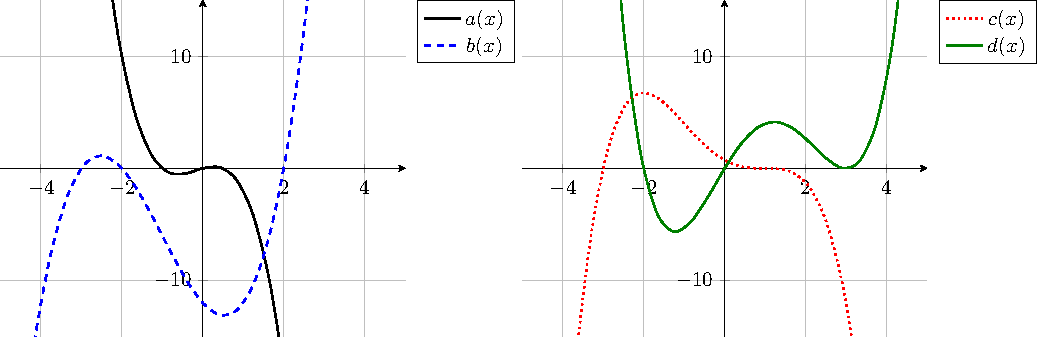
\includegraphics[width=0.99\columnwidth]{figures/0-6-fig6.pdf}
    \end{center}
\begin{exerciseSolution}
\end{exerciseSolution}


\item The cost in dollars for removing $p$ percent of pollutants from a river is 
    \[ C(p) = \frac{61700p}{100-p}. \]
    \ba
        \item Find the cost for removing 20\%.
        \item Find the cost for removing half of the pollutants.
        \item What is the smallest value $p$ can be?
        \item What is the largest value $p$ can be?
        \item What is the value of $C(p)$ as $p \to 100$?  What is the meaning of this in
            the context of the problem?
    \ea
\begin{exerciseSolution}
\end{exerciseSolution}

\item For the function 
    \[ f(x) = \frac{2x-6}{(-6x-1)(6x-6)}, \]
    \ba
        \item what are the vertical asymptotes?
        \item what are the horizontal asymptotes?
        \item what are the coordinates of the $x$ intercepts?
    \ea
\begin{exerciseSolution}
\end{exerciseSolution}

\item Square cuts of the same size are cut from a flat rectangular piece of cardboard. The
    remaining cardboard is folded into a lidless box. Assume that the cardboard originally
    measures 20 inches by 12 inches. Let $x$ be the length of one side of the square cut (at
    this point you should stop and draw a picture).
    \ba
        \item Write a function describing the volume of the resulting box in terms of $x$.
        \item What is an appropriate domain for the volume function?  Plot the volume function
            over the domain.
        \item Write a function describing the surface area of the box in terms of $x$.
        \item Is the domain different for the surface area function?  Why / why not?  Plot
            the surface area function over its appropriate domain.
    \ea

\end{exercises}
\afterexercises


\clearpage

 % Pre Calc topics
% \include{1.chap} % Understanding the Derivative
% \include{2.chap} % Computing derivatives
% \include{3.chap} % Using Derivatives
% \include{4.chap} % The Definite Integral
% \include{5.chap} % Finding Antiderivatives and Evaluating Integrals
% \include{6.chap} % Using Definite Integrals
% \include{7.chap} % Differential Equations
% \include{8.chap} % Sequences and Series
% 
% \include{9.chap} % Sequences, Difference Equations, and Discrete Dynamical Systems
% \include{10.chap} % Introduction to Linear Algebra
% 
% 
% \nocite{HughesHallet}
% \nocite{principles}
% \nocite{Arney}
% \nocite{nonlinear}
% \nocite{Noonburg}
% \nocite{Lay}
% 
% \pagebreak
% \bibliographystyle{plain}
% \bibliography{CarrollCalculusBib}
% \pagebreak
% 
%  \appendix
%  \include{A.Appendices}
% 
% \backmatter
% 	 
% \printindex

\end{document}
